\documentclass[11pt]{report}
\usepackage{./assignment2}
\usepackage{slashbox}
\usepackage{graphicx}
\usepackage{subfigure}
\usepackage{enumerate}
\usepackage[shortlabels]{enumitem}
\usepackage{stmaryrd}
\usepackage[final]{pdfpages}
\usepackage{array}
\usepackage{multirow}
\usepackage[T1]{fontenc}
\usepackage[utf8]{inputenc}
\usepackage{authblk}
\usepackage{amsmath}
\usepackage{amssymb}
\usepackage{epstopdf}
\usepackage{indentfirst}
\usepackage{bbm}
\usepackage{wrapfig}
\usepackage{biblatex}

\bibliography{references} 
%\bibliographystyle{unsrt}



\RequirePackage{latexsym}
\RequirePackage{amsmath}
\RequirePackage{amssymb}
\RequirePackage{bm}
\RequirePackage{url}
\RequirePackage{algorithmic}
\RequirePackage{algorithm2e}


%%%%%%%% Stock standard definitions %%%%%%%%%%%%%%%

%\newcommand{\ab}{\mathbf{a}}
%\newcommand{\bb}{\mathbf{b}}
%\newcommand{\cbb}{\mathbf{c}}
%\newcommand{\db}{\mathbf{d}}
%\newcommand{\eb}{\mathbf{e}}
%\newcommand{\fb}{\mathbf{f}}
%\newcommand{\gb}{\mathbf{g}}
%\newcommand{\hb}{\mathbf{h}}
%\newcommand{\ib}{\mathbf{i}}
%\newcommand{\jb}{\mathbf{j}}
%\newcommand{\kb}{\mathbf{k}}
%\newcommand{\lb}{\mathbf{l}}
%\newcommand{\mb}{\mathbf{m}}
%\newcommand{\nbb}{\mathbf{n}}
%\newcommand{\ob}{\mathbf{o}}
%\newcommand{\pb}{\mathbf{p}}
%\newcommand{\qb}{\mathbf{q}}
%\newcommand{\rb}{\mathbf{r}}
%\newcommand{\sbb}{\mathbf{s}}
%\newcommand{\tb}{\mathbf{t}}
%\newcommand{\ub}{\mathbf{u}}
%\newcommand{\vb}{\mathbf{v}}
%\newcommand{\wb}{\mathbf{w}}
%\newcommand{\xb}{\mathbf{x}}
%\newcommand{\yb}{\mathbf{y}}
%\newcommand{\zb}{\mathbf{z}}
%
%\newcommand{\abtil}{\tilde{\ab}}
%\newcommand{\bbtil}{\tilde{\bb}}
%\newcommand{\cbtil}{\tilde{\cbb}}
%\newcommand{\dbtil}{\tilde{\db}}
%\newcommand{\ebtil}{\tilde{\eb}}
%\newcommand{\fbtil}{\tilde{\fb}}
%\newcommand{\gbtil}{\tilde{\gb}}
%\newcommand{\hbtil}{\tilde{\hb}}
%\newcommand{\ibtil}{\tilde{\ib}}
%\newcommand{\jbtil}{\tilde{\jb}}
%\newcommand{\kbtil}{\tilde{\kb}}
%\newcommand{\lbtil}{\tilde{\lb}}
%\newcommand{\mbtil}{\tilde{\mb}}
%\newcommand{\nbtil}{\tilde{\nbb}}
%\newcommand{\obtil}{\tilde{\ob}}
%\newcommand{\pbtil}{\tilde{\pb}}
%\newcommand{\qbtil}{\tilde{\qb}}
%\newcommand{\rbtil}{\tilde{\rb}}
%\newcommand{\sbtil}{\tilde{\sbb}}
%\newcommand{\tbtil}{\tilde{\tb}}
%\newcommand{\ubtil}{\tilde{\ub}}
%\newcommand{\vbtil}{\tilde{\vb}}
%\newcommand{\wbtil}{\tilde{\wb}}
%\newcommand{\xbtil}{\tilde{\xb}}
%\newcommand{\ybtil}{\tilde{\yb}}
%\newcommand{\zbtil}{\tilde{\zb}}
%
%
%\newcommand{\atil}{\tilde{a}}
%\newcommand{\btil}{\tilde{b}}
%\newcommand{\ctil}{\tilde{c}}
%\newcommand{\dtil}{\tilde{d}}
%\newcommand{\etil}{\tilde{e}}
%\newcommand{\ftil}{\tilde{f}}
%\newcommand{\gtil}{\tilde{g}}
%\newcommand{\htil}{\tilde{h}}
%\newcommand{\itil}{\tilde{i}}
%\newcommand{\jtil}{\tilde{j}}
%\newcommand{\ktil}{\tilde{k}}
%\newcommand{\ltil}{\tilde{l}}
%\newcommand{\mtil}{\tilde{m}}
%\newcommand{\ntil}{\tilde{n}}
%\newcommand{\otil}{\tilde{o}}
%\newcommand{\ptil}{\tilde{p}}
%\newcommand{\qtil}{\tilde{q}}
%\newcommand{\rtil}{\tilde{r}}
%\newcommand{\stil}{\tilde{s}}
%\newcommand{\ttil}{\tilde{t}}
%\newcommand{\util}{\tilde{u}}
%\newcommand{\vtil}{\tilde{v}}
%\newcommand{\wtil}{\tilde{w}}
%\newcommand{\xtil}{\tilde{x}}
%\newcommand{\ytil}{\tilde{y}}
%\newcommand{\ztil}{\tilde{z}}
%
%\newcommand{\Atil}{\tilde{A}}
%\newcommand{\Btil}{\tilde{B}}
%\newcommand{\Ctil}{\tilde{C}}
%\newcommand{\Dtil}{\tilde{D}}
%\newcommand{\Etil}{\tilde{E}}
%\newcommand{\Ftil}{\tilde{F}}
%\newcommand{\Gtil}{\tilde{G}}
%\newcommand{\Htil}{\tilde{H}}
%\newcommand{\Itil}{\tilde{I}}
%\newcommand{\Jtil}{\tilde{J}}
%\newcommand{\Ktil}{\tilde{K}}
%\newcommand{\Ltil}{\tilde{L}}
%\newcommand{\Mtil}{\tilde{M}}
%\newcommand{\Ntil}{\tilde{N}}
%\newcommand{\Otil}{\tilde{O}}
%\newcommand{\Ptil}{\tilde{P}}
%\newcommand{\Qtil}{\tilde{Q}}
%\newcommand{\Rtil}{\tilde{R}}
%\newcommand{\Stil}{\tilde{S}}
%\newcommand{\Ttil}{\tilde{T}}
%\newcommand{\Util}{\tilde{U}}
%\newcommand{\Vtil}{\tilde{V}}
%\newcommand{\Wtil}{\tilde{W}}
%\newcommand{\Xtil}{\tilde{X}}
%\newcommand{\Ytil}{\tilde{Y}}
%\newcommand{\Ztil}{\tilde{Z}}
%
%\newcommand{\abar}{\bar{a}}
%\newcommand{\bbar}{\bar{b}}
%\newcommand{\cbar}{\bar{c}}
%\newcommand{\dbar}{\bar{d}}
%\newcommand{\ebar}{\bar{e}}
%\newcommand{\fbar}{\bar{f}}
%\newcommand{\gbar}{\bar{g}}
%\newcommand{\hbr}{\bar{h}}
%\newcommand{\ibar}{\bar{i}}
%\newcommand{\jbar}{\bar{j}}
%\newcommand{\kbar}{\bar{k}}
%\newcommand{\lbar}{\bar{l}}
%\newcommand{\mbar}{\bar{m}}
%\newcommand{\nbar}{\bar{n}}
%\newcommand{\obar}{\bar{o}}
%\newcommand{\pbar}{\bar{p}}
%\newcommand{\qbar}{\bar{q}}
%\newcommand{\rbar}{\bar{r}}
%\newcommand{\sbar}{\bar{s}}
%\newcommand{\tbar}{\bar{t}}
%\newcommand{\ubar}{\bar{u}}
%\newcommand{\vbar}{\bar{v}}
%\newcommand{\wbar}{\bar{w}}
%\newcommand{\xbar}{\bar{x}}
%\newcommand{\ybar}{\bar{y}}
%\newcommand{\zbar}{\bar{z}}
%
%\newcommand{\abbar}{\bar{\ab}}
%\newcommand{\bbbar}{\bar{\bb}}
%\newcommand{\cbbar}{\bar{\cb}}
%\newcommand{\dbbar}{\bar{\db}}
%\newcommand{\ebbar}{\bar{\eb}}
%\newcommand{\fbbar}{\bar{\fb}}
%\newcommand{\gbbar}{\bar{\gb}}
%\newcommand{\hbbar}{\bar{\hb}}
%\newcommand{\ibbar}{\bar{\ib}}
%\newcommand{\jbbar}{\bar{\jb}}
%\newcommand{\kbbar}{\bar{\kb}}
%\newcommand{\lbbar}{\bar{\lb}}
%\newcommand{\mbbar}{\bar{\mb}}
%\newcommand{\nbbar}{\bar{\nbb}}
%\newcommand{\obbar}{\bar{\ob}}
%\newcommand{\pbbar}{\bar{\pb}}
%\newcommand{\qbbar}{\bar{\qb}}
%\newcommand{\rbbar}{\bar{\rb}}
%\newcommand{\sbbar}{\bar{\sbb}}
%\newcommand{\tbbar}{\bar{\tb}}
%\newcommand{\ubbar}{\bar{\ub}}
%\newcommand{\vbbar}{\bar{\vb}}
%\newcommand{\wbbar}{\bar{\wb}}
%\newcommand{\xbbar}{\bar{\xb}}
%\newcommand{\ybbar}{\bar{\yb}}
%\newcommand{\zbbar}{\bar{\zb}}
%
%\newcommand{\Ab}{\mathbf{A}}
%\newcommand{\Bb}{\mathbf{B}}
%\newcommand{\Cb}{\mathbf{C}}
%\newcommand{\Db}{\mathbf{D}}
%\newcommand{\Eb}{\mathbf{E}}
%\newcommand{\Fb}{\mathbf{F}}
%\newcommand{\Gb}{\mathbf{G}}
%\newcommand{\Hb}{\mathbf{H}}
%\newcommand{\Ib}{\mathbf{I}}
%\newcommand{\Jb}{\mathbf{J}}
%\newcommand{\Kb}{\mathbf{K}}
%\newcommand{\Lb}{\mathbf{L}}
%\newcommand{\Mb}{\mathbf{M}}
%\newcommand{\Nb}{\mathbf{N}}
%\newcommand{\Ob}{\mathbf{O}}
%\newcommand{\Pb}{\mathbf{P}}
%\newcommand{\Qb}{\mathbf{Q}}
%\newcommand{\Rb}{\mathbf{R}}
%\newcommand{\Sbb}{\mathbf{S}}
%\newcommand{\Tb}{\mathbf{T}}
%\newcommand{\Ub}{\mathbf{U}}
%\newcommand{\Vb}{\mathbf{V}}
%\newcommand{\Wb}{\mathbf{W}}
%\newcommand{\Xb}{\mathbf{X}}
%\newcommand{\Yb}{\mathbf{Y}}
%\newcommand{\Zb}{\mathbf{Z}}
%
%\newcommand{\Abtil}{\tilde{\Ab}}
%\newcommand{\Bbtil}{\tilde{\Bb}}
%\newcommand{\Cbtil}{\tilde{\Cb}}
%\newcommand{\Dbtil}{\tilde{\Db}}
%\newcommand{\Ebtil}{\tilde{\Eb}}
%\newcommand{\Fbtil}{\tilde{\Fb}}
%\newcommand{\Gbtil}{\tilde{\Gb}}
%\newcommand{\Hbtil}{\tilde{\Hb}}
%\newcommand{\Ibtil}{\tilde{\Ib}}
%\newcommand{\Jbtil}{\tilde{\Jb}}
%\newcommand{\Kbtil}{\tilde{\Kb}}
%\newcommand{\Lbtil}{\tilde{\Lb}}
%\newcommand{\Mbtil}{\tilde{\Mb}}
%\newcommand{\Nbtil}{\tilde{\Nb}}
%\newcommand{\Obtil}{\tilde{\Ob}}
%\newcommand{\Pbtil}{\tilde{\Pb}}
%\newcommand{\Qbtil}{\tilde{\Qb}}
%\newcommand{\Rbtil}{\tilde{\Rb}}
%\newcommand{\Sbtil}{\tilde{\Sbb}}
%\newcommand{\Tbtil}{\tilde{\Tb}}
%\newcommand{\Ubtil}{\tilde{\Ub}}
%\newcommand{\Vbtil}{\tilde{\Vb}}
%\newcommand{\Wbtil}{\tilde{\Wb}}
%\newcommand{\Xbtil}{\tilde{\Xb}}
%\newcommand{\Ybtil}{\tilde{\Yb}}
%\newcommand{\Zbtil}{\tilde{\Zb}}
%
%\newcommand{\Abar}{\bar{A}}
%\newcommand{\Bbar}{\bar{B}}
%\newcommand{\Cbar}{\bar{C}}
%\newcommand{\Dbar}{\bar{D}}
%\newcommand{\Ebar}{\bar{E}}
%\newcommand{\Fbar}{\bar{F}}
%\newcommand{\Gbar}{\bar{G}}
%\newcommand{\Hbar}{\bar{H}}
%\newcommand{\Ibar}{\bar{I}}
%\newcommand{\Jbar}{\bar{J}}
%\newcommand{\Kbar}{\bar{K}}
%\newcommand{\Lbar}{\bar{L}}
%\newcommand{\Mbar}{\bar{M}}
%\newcommand{\Nbar}{\bar{N}}
%\newcommand{\Obar}{\bar{O}}
%\newcommand{\Pbar}{\bar{P}}
%\newcommand{\Qbar}{\bar{Q}}
%\newcommand{\Rbar}{\bar{R}}
%\newcommand{\Sbar}{\bar{S}}
%\newcommand{\Tbar}{\bar{T}}
%\newcommand{\Ubar}{\bar{U}}
%\newcommand{\Vbar}{\bar{V}}
%\newcommand{\Wbar}{\bar{W}}
%\newcommand{\Xbar}{\bar{X}}
%\newcommand{\Ybar}{\bar{Y}}
%\newcommand{\Zbar}{\bar{Z}}
%
%\newcommand{\Abbar}{\bar{\Ab}}
%\newcommand{\Bbbar}{\bar{\Bb}}
%\newcommand{\Cbbar}{\bar{\Cb}}
%\newcommand{\Dbbar}{\bar{\Db}}
%\newcommand{\Ebbar}{\bar{\Eb}}
%\newcommand{\Fbbar}{\bar{\Fb}}
%\newcommand{\Gbbar}{\bar{\Gb}}
%\newcommand{\Hbbar}{\bar{\Hb}}
%\newcommand{\Ibbar}{\bar{\Ib}}
%\newcommand{\Jbbar}{\bar{\Jb}}
%\newcommand{\Kbbar}{\bar{\Kb}}
%\newcommand{\Lbbar}{\bar{\Lb}}
%\newcommand{\Mbbar}{\bar{\Mb}}
%\newcommand{\Nbbar}{\bar{\Nb}}
%\newcommand{\Obbar}{\bar{\Ob}}
%\newcommand{\Pbbar}{\bar{\Pb}}
%\newcommand{\Qbbar}{\bar{\Qb}}
%\newcommand{\Rbbar}{\bar{\Rb}}
%\newcommand{\Sbbar}{\bar{\Sb}}
%\newcommand{\Tbbar}{\bar{\Tb}}
%\newcommand{\Ubbar}{\bar{\Ub}}
%\newcommand{\Vbbar}{\bar{\Vb}}
%\newcommand{\Wbbar}{\bar{\Wb}}
%\newcommand{\Xbbar}{\bar{\Xb}}
%\newcommand{\Ybbar}{\bar{\Yb}}
%\newcommand{\Zbbar}{\bar{\Zb}}
%
%\newcommand{\Ahat}{\hat{A}}
%\newcommand{\Bhat}{\hat{B}}
%\newcommand{\Chat}{\hat{C}}
%\newcommand{\Dhat}{\hat{D}}
%\newcommand{\Ehat}{\hat{E}}
%\newcommand{\Fhat}{\hat{F}}
%\newcommand{\Ghat}{\hat{G}}
%\newcommand{\Hhat}{\hat{H}}
%\newcommand{\Ihat}{\hat{I}}
%\newcommand{\Jhat}{\hat{J}}
%\newcommand{\Khat}{\hat{K}}
%\newcommand{\Lhat}{\hat{L}}
%\newcommand{\Mhat}{\hat{M}}
%\newcommand{\Nhat}{\hat{N}}
%\newcommand{\Ohat}{\hat{O}}
%\newcommand{\Phat}{\hat{P}}
%\newcommand{\Qhat}{\hat{Q}}
%\newcommand{\Rhat}{\hat{R}}
%\newcommand{\Shat}{\hat{S}}
%\newcommand{\That}{\hat{T}}
%\newcommand{\Uhat}{\hat{U}}
%\newcommand{\Vhat}{\hat{V}}
%\newcommand{\What}{\hat{W}}
%\newcommand{\Xhat}{\hat{X}}
%\newcommand{\Yhat}{\hat{Y}}
%\newcommand{\Zhat}{\hat{Z}}
%
%\newcommand{\Abhat}{\hat{\Ab}}
%\newcommand{\Bbhat}{\hat{\Bb}}
%\newcommand{\Cbhat}{\hat{\Cb}}
%\newcommand{\Dbhat}{\hat{\Db}}
%\newcommand{\Ebhat}{\hat{\Eb}}
%\newcommand{\Fbhat}{\hat{\Fb}}
%\newcommand{\Gbhat}{\hat{\Gb}}
%\newcommand{\Hbhat}{\hat{\Hb}}
%\newcommand{\Ibhat}{\hat{\Ib}}
%\newcommand{\Jbhat}{\hat{\Jb}}
%\newcommand{\Kbhat}{\hat{\Kb}}
%\newcommand{\Lbhat}{\hat{\Lb}}
%\newcommand{\Mbhat}{\hat{\Mb}}
%\newcommand{\Nbhat}{\hat{\Nb}}
%\newcommand{\Obhat}{\hat{\Ob}}
%\newcommand{\Pbhat}{\hat{\Pb}}
%\newcommand{\Qbhat}{\hat{\Qb}}
%\newcommand{\Rbhat}{\hat{\Rb}}
%\newcommand{\Sbhat}{\hat{\Sb}}
%\newcommand{\Tbhat}{\hat{\Tb}}
%\newcommand{\Ubhat}{\hat{\Ub}}
%\newcommand{\Vbhat}{\hat{\Vb}}
%\newcommand{\Wbhat}{\hat{\Wb}}
%\newcommand{\Xbhat}{\hat{\Xb}}
%\newcommand{\Ybhat}{\hat{\Yb}}
%\newcommand{\Zbhat}{\hat{\Zb}}
%
%\newcommand{\Acal}{\mathcal{A}}
%\newcommand{\Bcal}{\mathcal{B}}
%\newcommand{\Ccal}{\mathcal{C}}
%\newcommand{\Dcal}{\mathcal{D}}
%\newcommand{\Ecal}{\mathcal{E}}
%\newcommand{\Fcal}{\mathcal{F}}
%\newcommand{\Gcal}{\mathcal{G}}
%\newcommand{\Hcal}{\mathcal{H}}
%\newcommand{\Ical}{\mathcal{I}}
%\newcommand{\Jcal}{\mathcal{J}}
%\newcommand{\Kcal}{\mathcal{K}}
%\newcommand{\Lcal}{\mathcal{L}}
%\newcommand{\Mcal}{\mathcal{M}}
%\newcommand{\Ncal}{\mathcal{N}}
%\newcommand{\Ocal}{\mathcal{O}}
%\newcommand{\Pcal}{\mathcal{P}}
%\newcommand{\Qcal}{\mathcal{Q}}
%\newcommand{\Rcal}{\mathcal{R}}
%\newcommand{\Scal}{{\mathcal{S}}}
%\newcommand{\Tcal}{{\mathcal{T}}}
%\newcommand{\Ucal}{\mathcal{U}}
%\newcommand{\Vcal}{\mathcal{V}}
%\newcommand{\Wcal}{\mathcal{W}}
%\newcommand{\Xcal}{\mathcal{X}}
%\newcommand{\Ycal}{\mathcal{Y}}
%\newcommand{\Zcal}{\mathcal{Z}}
%
%\newcommand{\Atilde}{\widetilde{A}}
%\newcommand{\Btilde}{\widetilde{B}}
%\newcommand{\Ctilde}{\widetilde{C}}
%\newcommand{\Dtilde}{\widetilde{D}}
%\newcommand{\Etilde}{\widetilde{E}}
%\newcommand{\Ftilde}{\widetilde{F}}
%\newcommand{\Gtilde}{\widetilde{G}}
%\newcommand{\Htilde}{\widetilde{H}}
%\newcommand{\Itilde}{\widetilde{I}}
%\newcommand{\Jtilde}{\widetilde{J}}
%\newcommand{\Ktilde}{\widetilde{K}}
%\newcommand{\Ltilde}{\widetilde{L}}
%\newcommand{\Mtilde}{\widetilde{M}}
%\newcommand{\Ntilde}{\widetilde{N}}
%\newcommand{\Otilde}{\widetilde{O}}
%\newcommand{\Ptilde}{\widetilde{P}}
%\newcommand{\Qtilde}{\widetilde{Q}}
%\newcommand{\Rtilde}{\widetilde{R}}
%\newcommand{\Stilde}{\widetilde{S}}
%\newcommand{\Ttilde}{\widetilde{T}}
%\newcommand{\Utilde}{\widetilde{U}}
%\newcommand{\Vtilde}{\widetilde{V}}
%\newcommand{\Wtilde}{\widetilde{W}}
%\newcommand{\Xtilde}{\widetilde{X}}
%\newcommand{\Ytilde}{\widetilde{Y}}
%\newcommand{\Ztilde}{\widetilde{Z}}
%
%
%%%%%%%%% Widely accepted definitions %%%%%%%%%%%%%%%
%
%\newcommand{\CC}{\mathbb{C}} % Complex numbers
%\newcommand{\EE}{\mathbb{E}} % Expectation
%\newcommand{\II}{\mathbb{I}} % Delta Indicator
%\newcommand{\VV}{\mathbb{V}} % Variance
%\newcommand{\KK}{\mathbb{K}} % Arbitrary field
%\newcommand{\MM}{\mathbb{M}} % Median
%\newcommand{\NN}{\mathbb{N}} % Natural numbers
%\newcommand{\PP}{\mathbb{P}} % Probability
%\newcommand{\QQ}{\mathbb{Q}} % Rationals
%\newcommand{\RR}{\mathbb{R}} % Real numbers
%\newcommand{\ZZ}{\mathbb{Z}} % Integers
%\newcommand{\XX}{\mathbb{X}} % Integers
%\newcommand{\YY}{\mathbb{Y}} % Integers
%
%\newcommand{\one}{\mathbf{1}}  % Identity
%\newcommand{\zero}{\mathbf{0}} % Zero
%%\newcommand{\TRUE}{\mathbf{TRUE}}  % True
%%\newcommand{\FALSE}{\mathbf{FALSE}}  % False
%
%\newcommand*{\mini}{\mathop{\mathrm{minimize}}}
%\newcommand*{\maxi}{\mathop{\mathrm{maximize}}}
%\newcommand*{\argmin}{\mathop{\mathrm{argmin}}}
%\newcommand*{\argmax}{\mathop{\mathrm{argmax}}}
%\newcommand{\sgn}{\mathop{\mathrm{sign}}}
%\newcommand{\tr}{\mathop{\mathrm{tr}}}
%\newcommand{\diag}{\mathop{\mathrm{diag}}}
%\newcommand{\rank}{\mathop{\mathrm{rank}}}
%%\newcommand{\ovec}{\mathop{\mathrm{vec}}}
%\newcommand{\traj}{\mathop{\mathrm{Traj}}}
%\newcommand*{\cov}{\mathrm{Cov}}
%\newcommand*{\conv}{\mathrm{conv}}
%\newcommand*{\const}{\mathrm{constant}}
%
%%%%%%%%% Bold Greek Letters %%%%%%%%%%%%%%%
%\newcommand{\sigmab}{\bm{\sigma}}
%\newcommand{\Sigmab}{\mathbf{\Sigma}}
%
%
%%%%%%%%% Mess around with LaTeX %%%%%%%%%%%%%%%
%
%%% Some style files might actually define these variables.
%%% So don't mess with them if they are already defined
%
%\ifx\BlackBox\undefined
%\newcommand{\BlackBox}{\rule{1.5ex}{1.5ex}}  % end of proof
%\fi
%
%\ifx\QED\undefined
%\def\QED{~\rule[-1pt]{5pt}{5pt}\par\medskip}
%\fi
%
%\ifx\proof\undefined
%\newenvironment{proof}{\par\noindent{\bf Proof\ }}{\hfill\BlackBox\\[2mm]}
%%\newenvironment{proof}{\emph{Proof. }}{ \hfill \QED}
%\fi
%
%\ifx\theorem\undefined
%\newtheorem{theorem}{Theorem}
%\newtheorem{example}{Example}
%\newtheorem{property}{Property}
%\newtheorem{lemma}[theorem]{Lemma}
%\newtheorem{proposition}[theorem]{Proposition}
%\newtheorem{remark}[theorem]{Remark}
%\newtheorem{corollary}[theorem]{Corollary}
%\newtheorem{definition}[theorem]{Definition}
%\newtheorem{conjecture}[theorem]{Conjecture}
%\fi
%
%\ifx\axiom\undefined
%\newtheorem{axiom}[theorem]{Axiom}
%\fi
%
%%%%%%%%% Utility functions %%%%%%%%%%%%%%%
%
%\newcommand{\eq}[1]{(\ref{#1})}
%\newcommand{\mymatrix}[2]{\left[\begin{array}{#1} #2 \end{array}\right]}
%\newcommand{\mychoose}[2]{\left(\begin{array}{c} #1 \\ #2 \end{array}\right)}
%\newcommand{\mydet}[1]{\det\left[ #1 \right]}
%\newcommand{\sembrack}[1]{[\![#1]\!]}
%
%\newcommand{\ea}{\emph{et al.}}
%\newcommand{\eg}{\emph{e.g.}}
%\newcommand{\ie}{\emph{i.e.}}
%\newcommand{\iid}{\emph{iid}}
%
%%\newcommand{\alex}[1]{{\bf ALEX: \uppercase{#1}}}
%%\newcommand{\vishy}[1]{{\bf VISHY: \uppercase{#1}}}
%%\newcommand{\rene}[1]{{\bf RENE: \uppercase{#1}}}
%%\newcommand{\karsten}[1]{{\bf KARSTEN: \uppercase{#1}}}
%
%%%%%%%%% Specific symbols for this project %%%%%%%%%%%%%%%
%
%\newcommand{\methodname}{KDE}
%\newcommand{\ind}{\boldsymbol{\mathsf{I}}}
%
%\newcommand{\hsic}{\mathrm{HSIC}}
%\newcommand{\mmd}{\mathrm{MMD}}
%
%%\newcommand{\tDiag}{\textsf{Diag}}
%%\newcommand{\tTr}{\textsf{Tr}}
%%\newcommand{\tE}{\textsf{E}}
%%\newcommand{\tVec}{\textsf{Vec}}
%%\newcommand{\tRank}{\textsf{Rank}}
%
%%%%%%%%%%%%%%%%%%%%%%%%%%%%%%%%%%%%%%%%%%%%%%%%%%%%%%%%%%%%%%%%%%%%%%%%%%%%
%% math symbols and commands
%%%%%%%%%%%%%%%%%%%%%%%%%%%%%%%%%%%%%%%%%%%%%%%%%%%%%%%%%%%%%%%%%%%%%%%%%%%%
%%\newcommand{\eq}[1]{(\ref{#1})}
%%\newcommand{\mymatrix}[2]{\left[\begin{array}{#1} #2 \end{array}\right]}
%
%%brackets
%\newcommand{\inner}[2]{\left\langle #1,#2 \right\rangle}
%\newcommand{\rbr}[1]{\left(#1\right)}
%\newcommand{\sbr}[1]{\left[#1\right]}
%\newcommand{\cbr}[1]{\left\{#1\right\}}
%\newcommand{\nbr}[1]{\left\|#1\right\|}
%\newcommand{\abr}[1]{\left|#1\right|}
%\newcommand{\smallfrac}[2]{{\textstyle \frac{#1}{#2}}}
%\renewcommand{\url}[1]{{\sffamily #1}}
%\newcommand{\arow}[2]{#1_{#2\cdot}}
%\newcommand{\acol}[2]{#1_{\cdot#2}}
%
%\newcommand{\twoco}[1]{\multicolumn{2}{c|}{#1}}
%\def\ci{\perp\!\!\!\perp}
%
%
%%%% Local Variables:
%%%% mode: latex
%%%% TeX-master: "./SIGMOD06/SIGMODB06.tex"
%%%% End:
%
%
%% by xinhua
%\newcommand{\delhat}{\hat{\delta}}
%\newcommand{\delbar}{\bar{\delta}}
%\newcommand{\HH}{\mathbb{H}} % Arbitrary field
%\newcommand{\ve}{\varepsilon}
%\newcommand{\dom}{\mathrm{dom}}
%
%%%% Local Variables:
%%%% mode: latex
%%%% TeX-master: "./SIGMOD06/SIGMODB06.tex"
%%%% End:
%%%%%%%%%%%%%%%%%%%%%%%%%%%%%%%%%%%%%%%%%%%%%%%%%%%%%%%%%%%%%%%%%%%%%%%%%%%
%%                               PROOF, THEOREM, and FRIENDS
%%%%%%%%%%%%%%%%%%%%%%%%%%%%%%%%%%%%%%%%%%%%%%%%%%%%%%%%%%%%%%%%%%%%%%%%%%%%
%
%%\newcommand{\BlackBox}{\rule{1.5ex}{1.5ex}}  % end of proof
%%\newenvironment{proof}{\par\noindent{\bf Proof.\ }}{\hfill\BlackBox\\[2mm]}
%
%%\newcounter{all_counter}
%%\newcounter{lemma_counter}
%%\newcounter{proposition_counter}
%%\newcounter{remark_counter}
%%\newcounter{corollary_counter}
%%\newcounter{definition_counter}
%%\newcounter{conjecture_counter}
%%\newcounter{axiom_counter}
%%
%%\setcounter{lemma_counter}{0} \setcounter{proposition_counter}{0}
%%\setcounter{remark_counter}{0} \setcounter{corollary_counter}{0}
%%\setcounter{definition_counter}{0}
%%\setcounter{conjecture_counter}{0} \setcounter{axiom_counter}{0}
%
%%\newtheorem{lemma}[lemma_counter]{Lemma}
%%\newtheorem{proposition}[proposition_counter]{Proposition}
%%\newtheorem{remark}[remark_counter]{Remark}
%%\newtheorem{corollary}[corollary_counter]{Corollary}
%%\newtheorem{definition}[definition_counter]{Definition}
%%\newtheorem{conjecture}[conjecture_counter]{Conjecture}
%%\newtheorem{axiom}[axiom_counter]{Axiom}
%
%\newtheorem{assumption}[theorem]{Assumption}
%
%\newcommand{\ahat}{\hat{a}}
%\newcommand{\bhat}{\hat{b}}
%\newcommand{\chat}{\hat{c}}
%\newcommand{\dhat}{\hat{d}}
%\newcommand{\ehat}{\hat{e}}
%\newcommand{\fhat}{\hat{f}}
%\newcommand{\ghat}{\hat{g}}
%\newcommand{\hhat}{\hat{h}}
%\newcommand{\ihat}{\hat{i}}
%\newcommand{\jhat}{\hat{j}}
%\newcommand{\khat}{\hat{k}}
%\newcommand{\lhat}{\hat{l}}
%\newcommand{\mhat}{\hat{m}}
%\newcommand{\nhat}{\hat{n}}
%\newcommand{\ohat}{\hat{o}}
%\newcommand{\phat}{\hat{p}}
%\newcommand{\qhat}{\hat{q}}
%\newcommand{\rhat}{\hat{r}}
%\newcommand{\shat}{\hat{s}}
%\newcommand{\that}{\hat{t}}
%\newcommand{\uhat}{\hat{u}}
%\newcommand{\vhat}{\hat{v}}
%\newcommand{\what}{\hat{w}}
%\newcommand{\xhat}{\hat{x}}
%\newcommand{\yhat}{\hat{y}}
%\newcommand{\zhat}{\hat{z}}
%
%\newcommand{\abhat}{\hat{\ab}}
%\newcommand{\bbhat}{\hat{\bb}}
%\newcommand{\cbhat}{\hat{\cb}}
%\newcommand{\dbhat}{\hat{\db}}
%\newcommand{\ebhat}{\hat{\eb}}
%\newcommand{\fbhat}{\hat{\fb}}
%\newcommand{\gbhat}{\hat{\gb}}
%\newcommand{\hbhat}{\hat{\hb}}
%\newcommand{\ibhat}{\hat{\ib}}
%\newcommand{\jbhat}{\hat{\jb}}
%\newcommand{\kbhat}{\hat{\kb}}
%\newcommand{\lbhat}{\hat{\lb}}
%\newcommand{\mbhat}{\hat{\mb}}
%\newcommand{\nbhat}{\hat{\nb}}
%\newcommand{\obhat}{\hat{\ob}}
%\newcommand{\pbhat}{\hat{\pb}}
%\newcommand{\qbhat}{\hat{\qb}}
%\newcommand{\rbhat}{\hat{\rb}}
%\newcommand{\sbhat}{\hat{\sb}}
%\newcommand{\tbhat}{\hat{\tb}}
%\newcommand{\ubhat}{\hat{\ub}}
%\newcommand{\vbhat}{\hat{\vb}}
%\newcommand{\wbhat}{\hat{\wb}}
%\newcommand{\xbhat}{\hat{\xb}}
%\newcommand{\ybhat}{\hat{\yb}}
%\newcommand{\zbhat}{\hat{\zb}}
%
%\renewcommand{\vec}[1]{\mathbf{\boldsymbol{#1}}}
%
%\newcommand{\avec}{\vec{a}}
%\newcommand{\bvec}{\vec{b}}
%\newcommand{\cvec}{\vec{c}}
%\newcommand{\dvec}{\vec{d}}
%\newcommand{\evec}{\vec{e}}
%\newcommand{\fvec}{\vec{f}}
%\newcommand{\gvec}{\vec{g}}
%\newcommand{\hvec}{\vec{h}}
%\newcommand{\ivec}{\vec{i}}
%\newcommand{\jvec}{\vec{j}}
%\newcommand{\kvec}{\vec{k}}
%\newcommand{\lvec}{\vec{l}}
%\newcommand{\mvec}{\vec{m}}
%\newcommand{\nvec}{\vec{n}}
%\newcommand{\ovec}{\vec{o}}
%\newcommand{\pvec}{\vec{p}}
%\newcommand{\qvec}{\vec{q}}
%\newcommand{\rvec}{\vec{r}}
%\newcommand{\svec}{\vec{s}}
%\newcommand{\tvec}{\vec{t}}
%\newcommand{\uvec}{\vec{u}}
%\newcommand{\vvec}{\vec{v}}
%\newcommand{\wvec}{\vec{w}}
%\newcommand{\xvec}{\vec{x}}
%\newcommand{\yvec}{\vec{y}}
%\newcommand{\zvec}{\vec{z}}
%
%\newcommand{\Avec}{\vec{A}}
%\newcommand{\Bvec}{\vec{B}}
%\newcommand{\Cvec}{\vec{C}}
%\newcommand{\Dvec}{\vec{D}}
%\newcommand{\Evec}{\vec{E}}
%\newcommand{\Fvec}{\vec{F}}
%\newcommand{\Gvec}{\vec{G}}
%\newcommand{\Hvec}{\vec{H}}
%\newcommand{\Ivec}{\vec{I}}
%\newcommand{\Jvec}{\vec{J}}
%\newcommand{\Kvec}{\vec{K}}
%\newcommand{\Lvec}{\vec{L}}
%\newcommand{\Mvec}{\vec{M}}
%\newcommand{\Nvec}{\vec{N}}
%\newcommand{\Ovec}{\vec{O}}
%\newcommand{\Pvec}{\vec{P}}
%\newcommand{\Qvec}{\vec{Q}}
%\newcommand{\Rvec}{\vec{R}}
%\newcommand{\Svec}{\vec{S}}
%\newcommand{\Tvec}{\vec{T}}
%\newcommand{\Uvec}{\vec{U}}
%\newcommand{\Vvec}{\vec{V}}
%\newcommand{\Wvec}{\vec{W}}
%\newcommand{\Xvec}{\vec{X}}
%\newcommand{\Yvec}{\vec{Y}}
%\newcommand{\Zvec}{\vec{Z}}
%
%
%\newcommand{\alphavec}{\vec{\alpha}}
%\newcommand{\betavec}{\vec{\beta}}
%\newcommand{\deltavec}{\vec{\delta}}
%\newcommand{\etavec}{\vec{\eta}}
%\newcommand{\phivec}{\vec{\phi}}
%\newcommand{\psivec}{\vec{\psi}}
%\newcommand{\thetavec}{\vec{\theta}}
%\newcommand{\muvec}{\vec{\mu}}
%\newcommand{\xivec}{\vec{\xi}}
%
%
%\newcommand{\alphab}{\boldsymbol{\alpha}}
%\newcommand{\betab}{\boldsymbol{\beta}}
%\newcommand{\gammab}{\boldsymbol{\gamma}}
%\newcommand{\thetab}{\boldsymbol{\theta}}
%\newcommand{\mub}{\boldsymbol{\mu}}
%\newcommand{\xib}{\boldsymbol{\xi}}
%\newcommand{\Deltab}{\boldsymbol{\Delta}}
%\newcommand{\Pib}{\boldsymbol{\Pi}}
%\newcommand{\etab}{\boldsymbol{\eta}}
%\newcommand{\taub}{\boldsymbol{\tau}}
%\newcommand{\lambdab}{\boldsymbol{\lambda}}
%\newcommand{\pitil}{\tilde{\pi}}
%
%\newcommand{\rmd}{\mathrm{d}}
%\newcommand{\HSIC}{\mathrm{HSIC}}
%
%\newcommand{\dir}{\mathrm{Dir}}
%\newcommand{\dirp}{\mathrm{DP}}
%\newcommand{\multi}{\mathrm{Multi}}
%\newcommand{\gam}{\mathrm{Gamma}}
%\newcommand{\var}{\mathrm{Var}}
%\newcommand{\cor}{\mathrm{Corr}}
%\newcommand{\bet}{\mathrm{Beta}}
%
%\newcommand{\ra}{\rightarrow}
%
%\newcommand{\idf}{{\tt idf}}
%
%\newcommand{\tp}{\text{tp}}
%\newcommand{\fn}{\text{fn}}
%\newcommand{\fp}{\text{fp}}
%\newcommand{\tpb}{\overline{\text{tp}}}
%\newcommand{\fnb}{\overline{\text{fn}}}
%\newcommand{\fpb}{\overline{\text{fp}}}
%\newcommand{\pre}{\text{Pre}}
%\newcommand{\rec}{\text{Rec}}
%\newcommand{\fs}{\text{F-score}}
%\newcommand{\opt}{\text{opt}}
%
%\newcommand{\topics}{{\tt topics}}
%\newcommand{\industries}{{\tt industries}}
%\newcommand{\regions}{{\tt regions}}
%\newcommand{\ip}{{\tt ip}}
%\newcommand{\category}{{\tt category}}
%
%\newcommand{\grad}{{\nabla}}
%\newcommand{\gradbar}{{\bar{\nabla}}}
%\newcommand{\mbarr}{{\overline{M(r)}}}
%\newcommand{\card}{{\mathrm{card }}}
%\newcommand{\MED}{{\text{MED}}}
%\newcommand{\mubar}{\bar{\mu}}
%\newcommand{\emp}{{\mathrm{emp}}}
%\newcommand{\core}{{\mathrm{core}}}
%\newcommand{\zerob}{{\mathbf{0}}}
%\newcommand{\co}{{\mathrm{co}}}
%\newcommand{\argsup}{\mathop{\mathrm{argsup}}}
%\newcommand{\intr}{{\mathrm{int}}}
%\newcommand{\bd}{{\mathrm{bd}}}
%\newcommand{\BMRM}{{BMRM}}
%\newcommand{\where}{{\quad \text{where} \quad}}
%\newcommand{\lcg}{{\textit{l.c.g}}}
%\newcommand{\gradtil}{{\tilde{\grad}}}
%\newcommand{\alphabtil}{{\tilde{\alphab}}}
%\newcommand{\gstar}{{g^{\star}}}
%\newcommand{\fstar}{{f^{\star}}}
%
%
%\newcommand{\sqrttwo}{{\sqrt{2}}}
%\newcommand{\invsqrttwo}{{\frac{1}{\sqrt{2}}}}
%\newcommand{\invtwo}{{\frac{1}{2}}}
%\newcommand{\phihat}{{\hat{\phi}}}
%\newcommand{\cp}{\mathrm{cp}}
%\newcommand{\liblinear}{{\sf liblinear}}
%\newcommand{\lsbmrm}{{\sf ls-bmrm}}
%\newcommand{\qpbmrm}{{\sf qp-bmrm}}
%\newcommand{\pegasos}{{\sf pegasos}}
%\newcommand{\pegan}{{\sf pegasos-$n$}}
%\newcommand{\pegaone}{{\sf pegasos-1}}
%\newcommand{\nest}{{\sf Pragam}}
%\newcommand{\nestb}{{\sf Pragam-b}}
%\newcommand{\err}{{\sf err}}



\newcommand{\ab}{\mathbf{a}}
\newcommand{\bb}{\mathbf{b}}
\newcommand{\cbb}{\mathbf{c}}
\newcommand{\db}{\mathbf{d}}
\newcommand{\eb}{\mathbf{e}}
\newcommand{\fb}{\mathbf{f}}
\newcommand{\gb}{\mathbf{g}}
\newcommand{\hb}{\mathbf{h}}
\newcommand{\ib}{\mathbf{i}}
\newcommand{\jb}{\mathbf{j}}
\newcommand{\kb}{\mathbf{k}}
\newcommand{\lb}{\mathbf{l}}
\newcommand{\mb}{\mathbf{m}}
\newcommand{\nbb}{\mathbf{n}}
\newcommand{\ob}{\mathbf{o}}
\newcommand{\pb}{\mathbf{p}}
\newcommand{\qb}{\mathbf{q}}
\newcommand{\rb}{\mathbf{r}}
\newcommand{\sbb}{\mathbf{s}}
\newcommand{\tb}{\mathbf{t}}
\newcommand{\ub}{\mathbf{u}}
\newcommand{\vb}{\mathbf{v}}
\newcommand{\wb}{\mathbf{w}}
\newcommand{\xb}{\mathbf{x}}
\newcommand{\yb}{\mathbf{y}}
\newcommand{\zb}{\mathbf{z}}

\newcommand{\abtil}{\tilde{\ab}}
\newcommand{\bbtil}{\tilde{\bb}}
\newcommand{\cbtil}{\tilde{\cbb}}
\newcommand{\dbtil}{\tilde{\db}}
\newcommand{\ebtil}{\tilde{\eb}}
\newcommand{\fbtil}{\tilde{\fb}}
\newcommand{\gbtil}{\tilde{\gb}}
\newcommand{\hbtil}{\tilde{\hb}}
\newcommand{\ibtil}{\tilde{\ib}}
\newcommand{\jbtil}{\tilde{\jb}}
\newcommand{\kbtil}{\tilde{\kb}}
\newcommand{\lbtil}{\tilde{\lb}}
\newcommand{\mbtil}{\tilde{\mb}}
\newcommand{\nbtil}{\tilde{\nbb}}
\newcommand{\obtil}{\tilde{\ob}}
\newcommand{\pbtil}{\tilde{\pb}}
\newcommand{\qbtil}{\tilde{\qb}}
\newcommand{\rbtil}{\tilde{\rb}}
\newcommand{\sbtil}{\tilde{\sbb}}
\newcommand{\tbtil}{\tilde{\tb}}
\newcommand{\ubtil}{\tilde{\ub}}
\newcommand{\vbtil}{\tilde{\vb}}
\newcommand{\wbtil}{\tilde{\wb}}
\newcommand{\xbtil}{\tilde{\xb}}
\newcommand{\ybtil}{\tilde{\yb}}
\newcommand{\zbtil}{\tilde{\zb}}


\newcommand{\atil}{\tilde{a}}
\newcommand{\btil}{\tilde{b}}
\newcommand{\ctil}{\tilde{c}}
\newcommand{\dtil}{\tilde{d}}
\newcommand{\etil}{\tilde{e}}
\newcommand{\ftil}{\tilde{f}}
\newcommand{\gtil}{\tilde{g}}
\newcommand{\htil}{\tilde{h}}
\newcommand{\itil}{\tilde{i}}
\newcommand{\jtil}{\tilde{j}}
\newcommand{\ktil}{\tilde{k}}
\newcommand{\ltil}{\tilde{l}}
\newcommand{\mtil}{\tilde{m}}
\newcommand{\ntil}{\tilde{n}}
\newcommand{\otil}{\tilde{o}}
\newcommand{\ptil}{\tilde{p}}
\newcommand{\qtil}{\tilde{q}}
\newcommand{\rtil}{\tilde{r}}
\newcommand{\stil}{\tilde{s}}
\newcommand{\ttil}{\tilde{t}}
\newcommand{\util}{\tilde{u}}
\newcommand{\vtil}{\tilde{v}}
\newcommand{\wtil}{\tilde{w}}
\newcommand{\xtil}{\tilde{x}}
\newcommand{\ytil}{\tilde{y}}
\newcommand{\ztil}{\tilde{z}}

\newcommand{\Atil}{\tilde{A}}
\newcommand{\Btil}{\tilde{B}}
\newcommand{\Ctil}{\tilde{C}}
\newcommand{\Dtil}{\tilde{D}}
\newcommand{\Etil}{\tilde{E}}
\newcommand{\Ftil}{\tilde{F}}
\newcommand{\Gtil}{\tilde{G}}
\newcommand{\Htil}{\tilde{H}}
\newcommand{\Itil}{\tilde{I}}
\newcommand{\Jtil}{\tilde{J}}
\newcommand{\Ktil}{\tilde{K}}
\newcommand{\Ltil}{\tilde{L}}
\newcommand{\Mtil}{\tilde{M}}
\newcommand{\Ntil}{\tilde{N}}
\newcommand{\Otil}{\tilde{O}}
\newcommand{\Ptil}{\tilde{P}}
\newcommand{\Qtil}{\tilde{Q}}
\newcommand{\Rtil}{\tilde{R}}
\newcommand{\Stil}{\tilde{S}}
\newcommand{\Ttil}{\tilde{T}}
\newcommand{\Util}{\tilde{U}}
\newcommand{\Vtil}{\tilde{V}}
\newcommand{\Wtil}{\tilde{W}}
\newcommand{\Xtil}{\tilde{X}}
\newcommand{\Ytil}{\tilde{Y}}
\newcommand{\Ztil}{\tilde{Z}}

\newcommand{\abar}{\bar{a}}
\newcommand{\bbar}{\bar{b}}
\newcommand{\cbar}{\bar{c}}
\newcommand{\dbar}{\bar{d}}
\newcommand{\ebar}{\bar{e}}
\newcommand{\fbar}{\bar{f}}
\newcommand{\gbar}{\bar{g}}
\newcommand{\hbr}{\bar{h}}
\newcommand{\ibar}{\bar{i}}
\newcommand{\jbar}{\bar{j}}
\newcommand{\kbar}{\bar{k}}
\newcommand{\lbar}{\bar{l}}
\newcommand{\mbar}{\bar{m}}
\newcommand{\nbar}{\bar{n}}
\newcommand{\oobar}{\bar{o}}
\newcommand{\pbar}{\bar{p}}
\newcommand{\qbar}{\bar{q}}
\newcommand{\rbar}{\bar{r}}
\newcommand{\sbar}{\bar{s}}
\newcommand{\tbar}{\bar{t}}
\newcommand{\ubar}{\bar{u}}
\newcommand{\vbar}{\bar{v}}
\newcommand{\wbar}{\bar{w}}
\newcommand{\xbar}{\bar{x}}
\newcommand{\ybar}{\bar{y}}
\newcommand{\zbar}{\bar{z}}

\newcommand{\abbar}{\bar{\ab}}
\newcommand{\bbbar}{\bar{\bb}}
\newcommand{\cbbar}{\bar{\cb}}
\newcommand{\dbbar}{\bar{\db}}
\newcommand{\ebbar}{\bar{\eb}}
\newcommand{\fbbar}{\bar{\fb}}
\newcommand{\gbbar}{\bar{\gb}}
\newcommand{\hbbar}{\bar{\hb}}
\newcommand{\ibbar}{\bar{\ib}}
\newcommand{\jbbar}{\bar{\jb}}
\newcommand{\kbbar}{\bar{\kb}}
\newcommand{\lbbar}{\bar{\lb}}
\newcommand{\mbbar}{\bar{\mb}}
\newcommand{\nbbar}{\bar{\nbb}}
\newcommand{\obbar}{\bar{\ob}}
\newcommand{\pbbar}{\bar{\pb}}
\newcommand{\qbbar}{\bar{\qb}}
\newcommand{\rbbar}{\bar{\rb}}
\newcommand{\sbbar}{\bar{\sbb}}
\newcommand{\tbbar}{\bar{\tb}}
\newcommand{\ubbar}{\bar{\ub}}
\newcommand{\vbbar}{\bar{\vb}}
\newcommand{\wbbar}{\bar{\wb}}
\newcommand{\xbbar}{\bar{\xb}}
\newcommand{\ybbar}{\bar{\yb}}
\newcommand{\zbbar}{\bar{\zb}}

\newcommand{\Ab}{\mathbf{A}}
\newcommand{\Bb}{\mathbf{B}}
\newcommand{\Cb}{\mathbf{C}}
\newcommand{\Db}{\mathbf{D}}
\newcommand{\Eb}{\mathbf{E}}
\newcommand{\Fb}{\mathbf{F}}
\newcommand{\Gb}{\mathbf{G}}
\newcommand{\Hb}{\mathbf{H}}
\newcommand{\Ib}{\mathbf{I}}
\newcommand{\Jb}{\mathbf{J}}
\newcommand{\Kb}{\mathbf{K}}
\newcommand{\Lb}{\mathbf{L}}
\newcommand{\Mb}{\mathbf{M}}
\newcommand{\Nb}{\mathbf{N}}
\newcommand{\Ob}{\mathbf{O}}
\newcommand{\Pb}{\mathbf{P}}
\newcommand{\Qb}{\mathbf{Q}}
\newcommand{\Rb}{\mathbf{R}}
\newcommand{\Sbb}{\mathbf{S}}
\newcommand{\Tb}{\mathbf{T}}
\newcommand{\Ub}{\mathbf{U}}
\newcommand{\Vb}{\mathbf{V}}
\newcommand{\Wb}{\mathbf{W}}
\newcommand{\Xb}{\mathbf{X}}
\newcommand{\Yb}{\mathbf{Y}}
\newcommand{\Zb}{\mathbf{Z}}

\newcommand{\Abtil}{\tilde{\Ab}}
\newcommand{\Bbtil}{\tilde{\Bb}}
\newcommand{\Cbtil}{\tilde{\Cb}}
\newcommand{\Dbtil}{\tilde{\Db}}
\newcommand{\Ebtil}{\tilde{\Eb}}
\newcommand{\Fbtil}{\tilde{\Fb}}
\newcommand{\Gbtil}{\tilde{\Gb}}
\newcommand{\Hbtil}{\tilde{\Hb}}
\newcommand{\Ibtil}{\tilde{\Ib}}
\newcommand{\Jbtil}{\tilde{\Jb}}
\newcommand{\Kbtil}{\tilde{\Kb}}
\newcommand{\Lbtil}{\tilde{\Lb}}
\newcommand{\Mbtil}{\tilde{\Mb}}
\newcommand{\Nbtil}{\tilde{\Nb}}
\newcommand{\Obtil}{\tilde{\Ob}}
\newcommand{\Pbtil}{\tilde{\Pb}}
\newcommand{\Qbtil}{\tilde{\Qb}}
\newcommand{\Rbtil}{\tilde{\Rb}}
\newcommand{\Sbtil}{\tilde{\Sbb}}
\newcommand{\Tbtil}{\tilde{\Tb}}
\newcommand{\Ubtil}{\tilde{\Ub}}
\newcommand{\Vbtil}{\tilde{\Vb}}
\newcommand{\Wbtil}{\tilde{\Wb}}
\newcommand{\Xbtil}{\tilde{\Xb}}
\newcommand{\Ybtil}{\tilde{\Yb}}
\newcommand{\Zbtil}{\tilde{\Zb}}

\newcommand{\Abar}{\bar{A}}
\newcommand{\Bbar}{\bar{B}}
\newcommand{\Cbar}{\bar{C}}
\newcommand{\Dbar}{\bar{D}}
\newcommand{\Ebar}{\bar{E}}
\newcommand{\Fbar}{\bar{F}}
\newcommand{\Gbar}{\bar{G}}
\newcommand{\Hbar}{\bar{H}}
\newcommand{\Ibar}{\bar{I}}
\newcommand{\Jbar}{\bar{J}}
\newcommand{\Kbar}{\bar{K}}
\newcommand{\Lbar}{\bar{L}}
\newcommand{\Mbar}{\bar{M}}
\newcommand{\Nbar}{\bar{N}}
\newcommand{\Obar}{\bar{O}}
\newcommand{\Pbar}{\bar{P}}
\newcommand{\Qbar}{\bar{Q}}
\newcommand{\Rbar}{\bar{R}}
\newcommand{\Sbar}{\bar{S}}
\newcommand{\Tbar}{\bar{T}}
\newcommand{\Ubar}{\bar{U}}
\newcommand{\Vbar}{\bar{V}}
\newcommand{\Wbar}{\bar{W}}
\newcommand{\Xbar}{\bar{X}}
\newcommand{\Ybar}{\bar{Y}}
\newcommand{\Zbar}{\bar{Z}}

\newcommand{\Abbar}{\bar{\Ab}}
\newcommand{\Bbbar}{\bar{\Bb}}
\newcommand{\Cbbar}{\bar{\Cb}}
\newcommand{\Dbbar}{\bar{\Db}}
\newcommand{\Ebbar}{\bar{\Eb}}
\newcommand{\Fbbar}{\bar{\Fb}}
\newcommand{\Gbbar}{\bar{\Gb}}
\newcommand{\Hbbar}{\bar{\Hb}}
\newcommand{\Ibbar}{\bar{\Ib}}
\newcommand{\Jbbar}{\bar{\Jb}}
\newcommand{\Kbbar}{\bar{\Kb}}
\newcommand{\Lbbar}{\bar{\Lb}}
\newcommand{\Mbbar}{\bar{\Mb}}
\newcommand{\Nbbar}{\bar{\Nb}}
\newcommand{\Obbar}{\bar{\Ob}}
\newcommand{\Pbbar}{\bar{\Pb}}
\newcommand{\Qbbar}{\bar{\Qb}}
\newcommand{\Rbbar}{\bar{\Rb}}
\newcommand{\Sbbar}{\bar{\Sb}}
\newcommand{\Tbbar}{\bar{\Tb}}
\newcommand{\Ubbar}{\bar{\Ub}}
\newcommand{\Vbbar}{\bar{\Vb}}
\newcommand{\Wbbar}{\bar{\Wb}}
\newcommand{\Xbbar}{\bar{\Xb}}
\newcommand{\Ybbar}{\bar{\Yb}}
\newcommand{\Zbbar}{\bar{\Zb}}

\newcommand{\Ahat}{\hat{A}}
\newcommand{\Bhat}{\hat{B}}
\newcommand{\Chat}{\hat{C}}
\newcommand{\Dhat}{\hat{D}}
\newcommand{\Ehat}{\hat{E}}
\newcommand{\Fhat}{\hat{F}}
\newcommand{\Ghat}{\hat{G}}
\newcommand{\Hhat}{\hat{H}}
\newcommand{\Ihat}{\hat{I}}
\newcommand{\Jhat}{\hat{J}}
\newcommand{\Khat}{\hat{K}}
\newcommand{\Lhat}{\hat{L}}
\newcommand{\Mhat}{\hat{M}}
\newcommand{\Nhat}{\hat{N}}
\newcommand{\Ohat}{\hat{O}}
\newcommand{\Phat}{\hat{P}}
\newcommand{\Qhat}{\hat{Q}}
\newcommand{\Rhat}{\hat{R}}
\newcommand{\Shat}{\hat{S}}
\newcommand{\That}{\hat{T}}
\newcommand{\Uhat}{\hat{U}}
\newcommand{\Vhat}{\hat{V}}
\newcommand{\What}{\hat{W}}
\newcommand{\Xhat}{\hat{X}}
\newcommand{\Yhat}{\hat{Y}}
\newcommand{\Zhat}{\hat{Z}}

\newcommand{\Abhat}{\hat{\Ab}}
\newcommand{\Bbhat}{\hat{\Bb}}
\newcommand{\Cbhat}{\hat{\Cb}}
\newcommand{\Dbhat}{\hat{\Db}}
\newcommand{\Ebhat}{\hat{\Eb}}
\newcommand{\Fbhat}{\hat{\Fb}}
\newcommand{\Gbhat}{\hat{\Gb}}
\newcommand{\Hbhat}{\hat{\Hb}}
\newcommand{\Ibhat}{\hat{\Ib}}
\newcommand{\Jbhat}{\hat{\Jb}}
\newcommand{\Kbhat}{\hat{\Kb}}
\newcommand{\Lbhat}{\hat{\Lb}}
\newcommand{\Mbhat}{\hat{\Mb}}
\newcommand{\Nbhat}{\hat{\Nb}}
\newcommand{\Obhat}{\hat{\Ob}}
\newcommand{\Pbhat}{\hat{\Pb}}
\newcommand{\Qbhat}{\hat{\Qb}}
\newcommand{\Rbhat}{\hat{\Rb}}
\newcommand{\Sbhat}{\hat{\Sb}}
\newcommand{\Tbhat}{\hat{\Tb}}
\newcommand{\Ubhat}{\hat{\Ub}}
\newcommand{\Vbhat}{\hat{\Vb}}
\newcommand{\Wbhat}{\hat{\Wb}}
\newcommand{\Xbhat}{\hat{\Xb}}
\newcommand{\Ybhat}{\hat{\Yb}}
\newcommand{\Zbhat}{\hat{\Zb}}

\newcommand{\Acal}{\mathcal{A}}
\newcommand{\Bcal}{\mathcal{B}}
\newcommand{\Ccal}{\mathcal{C}}
\newcommand{\Dcal}{\mathcal{D}}
\newcommand{\Ecal}{\mathcal{E}}
\newcommand{\Fcal}{\mathcal{F}}
\newcommand{\Gcal}{\mathcal{G}}
\newcommand{\Hcal}{\mathcal{H}}
\newcommand{\Ical}{\mathcal{I}}
\newcommand{\Jcal}{\mathcal{J}}
\newcommand{\Kcal}{\mathcal{K}}
\newcommand{\Lcal}{\mathcal{L}}
\newcommand{\Mcal}{\mathcal{M}}
\newcommand{\Ncal}{\mathcal{N}}
\newcommand{\Ocal}{\mathcal{O}}
\newcommand{\Pcal}{\mathcal{P}}
\newcommand{\Qcal}{\mathcal{Q}}
\newcommand{\Rcal}{\mathcal{R}}
\newcommand{\Scal}{{\mathcal{S}}}
\newcommand{\Tcal}{{\mathcal{T}}}
\newcommand{\Ucal}{\mathcal{U}}
\newcommand{\Vcal}{\mathcal{V}}
\newcommand{\Wcal}{\mathcal{W}}
\newcommand{\Xcal}{\mathcal{X}}
\newcommand{\Ycal}{\mathcal{Y}}
\newcommand{\Zcal}{\mathcal{Z}}

\newcommand{\Atilde}{\widetilde{A}}
\newcommand{\Btilde}{\widetilde{B}}
\newcommand{\Ctilde}{\widetilde{C}}
\newcommand{\Dtilde}{\widetilde{D}}
\newcommand{\Etilde}{\widetilde{E}}
\newcommand{\Ftilde}{\widetilde{F}}
\newcommand{\Gtilde}{\widetilde{G}}
\newcommand{\Htilde}{\widetilde{H}}
\newcommand{\Itilde}{\widetilde{I}}
\newcommand{\Jtilde}{\widetilde{J}}
\newcommand{\Ktilde}{\widetilde{K}}
\newcommand{\Ltilde}{\widetilde{L}}
\newcommand{\Mtilde}{\widetilde{M}}
\newcommand{\Ntilde}{\widetilde{N}}
\newcommand{\Otilde}{\widetilde{O}}
\newcommand{\Ptilde}{\widetilde{P}}
\newcommand{\Qtilde}{\widetilde{Q}}
\newcommand{\Rtilde}{\widetilde{R}}
\newcommand{\Stilde}{\widetilde{S}}
\newcommand{\Ttilde}{\widetilde{T}}
\newcommand{\Utilde}{\widetilde{U}}
\newcommand{\Vtilde}{\widetilde{V}}
\newcommand{\Wtilde}{\widetilde{W}}
\newcommand{\Xtilde}{\widetilde{X}}
\newcommand{\Ytilde}{\widetilde{Y}}
\newcommand{\Ztilde}{\widetilde{Z}}

\newcommand{\ahat}{\hat{a}}
\newcommand{\bhat}{\hat{b}}
\newcommand{\chat}{\hat{c}}
\newcommand{\dhat}{\hat{d}}
\newcommand{\ehat}{\hat{e}}
\newcommand{\fhat}{\hat{f}}
\newcommand{\ghat}{\hat{g}}
\newcommand{\hhat}{\hat{h}}
\newcommand{\ihat}{\hat{i}}
\newcommand{\jhat}{\hat{j}}
\newcommand{\khat}{\hat{k}}
\newcommand{\lhat}{\hat{l}}
\newcommand{\mhat}{\hat{m}}
\newcommand{\nhat}{\hat{n}}
\newcommand{\ohat}{\hat{o}}
\newcommand{\phat}{\hat{p}}
\newcommand{\qhat}{\hat{q}}
\newcommand{\rhat}{\hat{r}}
\newcommand{\shat}{\hat{s}}
\newcommand{\that}{\hat{t}}
\newcommand{\uhat}{\hat{u}}
\newcommand{\vhat}{\hat{v}}
\newcommand{\what}{\hat{w}}
\newcommand{\xhat}{\hat{x}}
\newcommand{\yhat}{\hat{y}}
\newcommand{\zhat}{\hat{z}}

\newcommand{\abhat}{\hat{\ab}}
\newcommand{\bbhat}{\hat{\bb}}
\newcommand{\cbhat}{\hat{\cb}}
\newcommand{\dbhat}{\hat{\db}}
\newcommand{\ebhat}{\hat{\eb}}
\newcommand{\fbhat}{\hat{\fb}}
\newcommand{\gbhat}{\hat{\gb}}
\newcommand{\hbhat}{\hat{\hb}}
\newcommand{\ibhat}{\hat{\ib}}
\newcommand{\jbhat}{\hat{\jb}}
\newcommand{\kbhat}{\hat{\kb}}
\newcommand{\lbhat}{\hat{\lb}}
\newcommand{\mbhat}{\hat{\mb}}
\newcommand{\nbhat}{\hat{\nb}}
\newcommand{\obhat}{\hat{\ob}}
\newcommand{\pbhat}{\hat{\pb}}
\newcommand{\qbhat}{\hat{\qb}}
\newcommand{\rbhat}{\hat{\rb}}
\newcommand{\sbhat}{\hat{\sb}}
\newcommand{\tbhat}{\hat{\tb}}
\newcommand{\ubhat}{\hat{\ub}}
\newcommand{\vbhat}{\hat{\vb}}
\newcommand{\wbhat}{\hat{\wb}}
\newcommand{\xbhat}{\hat{\xb}}
\newcommand{\ybhat}{\hat{\yb}}
\newcommand{\zbhat}{\hat{\zb}}




\renewcommand{\vec}[1]{\mathbf{\boldsymbol{#1}}}

\newcommand{\avec}{\vec{a}}
\newcommand{\bvec}{\vec{b}}
\newcommand{\cvec}{\vec{c}}
\newcommand{\dvec}{\vec{d}}
\newcommand{\evec}{\vec{e}}
\newcommand{\fvec}{\vec{f}}
\newcommand{\gvec}{\vec{g}}
\newcommand{\hvec}{\vec{h}}
\newcommand{\ivec}{\vec{i}}
\newcommand{\jvec}{\vec{j}}
\newcommand{\kvec}{\vec{k}}
\newcommand{\lvec}{\vec{l}}
\newcommand{\mvec}{\vec{m}}
\newcommand{\nvec}{\vec{n}}
\newcommand{\ovec}{\vec{o}}
\newcommand{\pvec}{\vec{p}}
\newcommand{\qvec}{\vec{q}}
\newcommand{\rvec}{\vec{r}}
\newcommand{\svec}{\vec{s}}
\newcommand{\tvec}{\vec{t}}
\newcommand{\uvec}{\vec{u}}
\newcommand{\vvec}{\vec{v}}
\newcommand{\wvec}{\vec{w}}
\newcommand{\xvec}{\vec{x}}
\newcommand{\yvec}{\vec{y}}
\newcommand{\zvec}{\vec{z}}

\newcommand{\Avec}{\vec{A}}
\newcommand{\Bvec}{\vec{B}}
\newcommand{\Cvec}{\vec{C}}
\newcommand{\Dvec}{\vec{D}}
\newcommand{\Evec}{\vec{E}}
\newcommand{\Fvec}{\vec{F}}
\newcommand{\Gvec}{\vec{G}}
\newcommand{\Hvec}{\vec{H}}
\newcommand{\Ivec}{\vec{I}}
\newcommand{\Jvec}{\vec{J}}
\newcommand{\Kvec}{\vec{K}}
\newcommand{\Lvec}{\vec{L}}
\newcommand{\Mvec}{\vec{M}}
\newcommand{\Nvec}{\vec{N}}
\newcommand{\Ovec}{\vec{O}}
\newcommand{\Pvec}{\vec{P}}
\newcommand{\Qvec}{\vec{Q}}
\newcommand{\Rvec}{\vec{R}}
\newcommand{\Svec}{\vec{S}}
\newcommand{\Tvec}{\vec{T}}
\newcommand{\Uvec}{\vec{U}}
\newcommand{\Vvec}{\vec{V}}
\newcommand{\Wvec}{\vec{W}}
\newcommand{\Xvec}{\vec{X}}
\newcommand{\Yvec}{\vec{Y}}
\newcommand{\Zvec}{\vec{Z}}

\newcommand{\wvechat}{\hat{\vec{w}}}

\newcommand{\alphavec}{\vec{\alpha}}
\newcommand{\alphavecbar}{\bar{\vec{\alpha}}}
\newcommand{\alphavechat}{\hat{\vec{\alpha}}}
\newcommand{\alphavectil}{\tilde{\vec{\alpha}}}
\newcommand{\betavec}{\vec{\beta}}
\newcommand{\deltavec}{\vec{\delta}}
\newcommand{\etavec}{\vec{\eta}}
\newcommand{\phivec}{\vec{\phi}}
\newcommand{\psivec}{\vec{\psi}}
\newcommand{\thetavec}{\vec{\theta}}
\newcommand{\muvec}{\vec{\mu}}
\newcommand{\xivec}{\vec{\xi}}



\newcommand{\va}{{\tt a}}
\newcommand{\vc}{{\tt c}}
\newcommand{\vg}{{\tt g}}
\newcommand{\vp}{{\tt p}}
\newcommand{\vq}{{\tt q}}
\newcommand{\vs}{{\tt s}}
\newcommand{\vt}{{\tt t}}
\newcommand{\vu}{{\tt u}}
\newcommand{\vv}{{\tt v}}
\newcommand{\vw}{{\tt w}}
\newcommand{\vx}{{\tt x}}
\newcommand{\vy}{{\tt y}}
\newcommand{\val}{{\tt v}}


\newcommand{\Amat}{\Ab}
\newcommand{\Bmat}{\Bb}
\newcommand{\Cmat}{\Cb}
\newcommand{\Dmat}{\Db}
\newcommand{\Emat}{\Eb}
\newcommand{\Fmat}{\Fb}
\newcommand{\Gmat}{\Gb}
\newcommand{\Hmat}{\Hb}
\newcommand{\Imat}{\Ib}

\newcommand{\Vmat}{\Vb}
\newcommand{\Wmat}{\Wb}
\newcommand{\Xmat}{\Xb}
\newcommand{\Ymat}{\Yb}
\newcommand{\Zmat}{\Zb}


%%%%%%%% Greek letters definitions %%%%%%%%%%%%%%%
\newcommand{\delhat}{\hat{\delta}}
\newcommand{\delbar}{\bar{\delta}}
\newcommand{\ve}{\varepsilon}
\newcommand{\epsilonbar}{\bar{\epsilon}}
\newcommand{\etabar}{\bar{\eta}}
\newcommand{\Omegahat}{\hat{\Omega}}

\newcommand{\alphab}{\boldsymbol{\alpha}}
\newcommand{\betab}{\boldsymbol{\beta}}
\newcommand{\gammab}{\boldsymbol{\gamma}}
\newcommand{\Gammab}{\boldsymbol{\Gamma}}
\newcommand{\thetab}{\boldsymbol{\theta}}
\newcommand{\mub}{\boldsymbol{\mu}}
\newcommand{\phib}{\boldsymbol{\phi}}
\newcommand{\Deltab}{\boldsymbol{\Delta}}
\newcommand{\xib}{\boldsymbol{\xi}}
\newcommand{\lambdab}{\boldsymbol{\lambda}}
\newcommand{\Pib}{\boldsymbol{\Pi}}
\newcommand{\etab}{\boldsymbol{\eta}}
\newcommand{\taub}{\boldsymbol{\tau}}
\newcommand{\rhob}{\boldsymbol{\rho}}
\newcommand{\sigmab}{\boldsymbol{\sigma}}
\newcommand{\Sigmab}{\boldsymbol{\Sigma}}

\newcommand{\thetatil}{\tilde{\theta}}
\newcommand{\pitil}{\tilde{\pi}}


%%%%%%%% Mathematical definitions %%%%%%%%%%%%%%%

\newcommand{\CC}{\mathbb{C}} % Complex numbers
\newcommand{\EE}{\mathbb{E}} % Expectation
\newcommand{\HH}{\mathbb{H}} % Arbitrary field
\newcommand{\II}{\mathbb{I}} % Delta Indicator
\newcommand{\VV}{\mathbb{V}} % Variance
\newcommand{\KK}{\mathbb{K}} % Arbitrary field
\newcommand{\MM}{\mathbb{M}} % Median
\newcommand{\NN}{\mathbb{N}} % Natural numbers
\newcommand{\PP}{\mathbb{P}} % Probability
\newcommand{\QQ}{\mathbb{Q}} % Rationals
\newcommand{\RR}{\mathbb{R}} % Real numbers
\newcommand{\RRbar}{\overline{\mathbb{R}}} % Real numbers
\newcommand{\ZZ}{\mathbb{Z}} % Integers
\newcommand{\XX}{\mathbb{X}} % Integers
\newcommand{\YY}{\mathbb{Y}} % Integers

%%%%%%%%%%%%%%%  Mathematical Constants  %%%%%%%%%%%%%%%
\newcommand{\one}{\mathbf{1}}  % Identity
\newcommand{\zero}{\mathbf{0}} % Zero
\newcommand{\vone}{\mathbf{1}}  % Identity
\newcommand{\vzero}{\mathbf{0}} % Zero
\newcommand{\ind}{\boldsymbol{\mathsf{I}}}
\newcommand{\half}{\frac{1}{2}}
\newcommand{\sqrttwo}{\sqrt{2}}
\newcommand{\invsqrttwo}{\frac{1}{\sqrt{2}}}
\newcommand{\invtwo}{\frac{1}{2}}





%\newcommand{\TRUE}{\mathbf{TRUE}}  % True
%\newcommand{\FALSE}{\mathbf{FALSE}}  % False


%%%%%%%%%%%%%  Mathematical Operators  %%%%%%%%%%%%%%%

\DeclareMathOperator*{\mini}{\mathrm{minimize}}
\DeclareMathOperator*{\maxi}{\mathrm{maximize}}
\DeclareMathOperator*{\argmin}{\mathrm{argmin}}
\DeclareMathOperator*{\argmax}{\mathrm{argmax}}
\DeclareMathOperator*{\arginf}{\mathrm{arginf}}
\DeclareMathOperator*{\argsup}{\mathrm{argsup}}



%\newcommand*{\argmin}{\mathop{\mathrm{argmin}}}
%\newcommand*{\argmax}{\mathop{\mathrm{argmax}}}
%\newcommand*{\arginf}{\mathop{\mathrm{arginf}}}
%\newcommand*{\argsup}{\mathop{\mathrm{argsup}}}
%\newcommand{\sgn}{\mathop{\mathrm{sign}}}
%\newcommand{\tr}{\mathop{\mathrm{tr}}}
\newcommand{\trace}{\mathop{\mathrm{tr}}}
\newcommand{\diag}{\mathop{\mathrm{diag}}}
%\newcommand{\rank}{\mathop{\mathrm{rank}}}
\newcommand{\opvec}{\mathop{\mathrm{vec}}}
%\newcommand{\traj}{\mathop{\mathrm{Traj}}}
\newcommand*{\cov}{\mathrm{Cov}}
\newcommand*{\covars}{\mathrm{Cov}}
\newcommand*{\conv}{\mathrm{conv}}
\newcommand*{\const}{\mathrm{constant}}
%\newcommand{\tDiag}{\textsf{Diag}}
%\newcommand{\tTr}{\textsf{Tr}}
%\newcommand{\tE}{\textsf{E}}
%\newcommand{\tVec}{\textsf{Vec}}
%\newcommand{\tRank}{\textsf{Rank}}
\DeclareMathOperator{\sgn}{\mathop{\mathrm{sign}}}
\DeclareMathOperator{\tr}{\mathop{\mathrm{tr}}}
\DeclareMathOperator{\rank}{\mathop{\mathrm{rank}}}
\DeclareMathOperator{\traj}{\mathop{\mathrm{Traj}}}
\providecommand{\tra}{\intercal}
\newcommand{\ra}{\rightarrow}
\newcommand{\totvar}{\mathrm{TV}}


%%%%%%%% Thorems, Corollaries, etc %%%%%%%%%%%%%%%

%% Some style files might actually define these variables.
%% So don't mess with them if they are already defined

\ifx\BlackBox\undefined
\newcommand{\BlackBox}{\rule{1.5ex}{1.5ex}}  % end of proof
\fi

\ifx\QED\undefined
\def\QED{~\rule[-1pt]{5pt}{5pt}\par\medskip}
\fi

\ifx\proof\undefined
\newenvironment{proof}{\par\noindent{\bf Proof\ }}{\hfill\BlackBox\\[2mm]}
%\newenvironment{proof}{\emph{Proof. }}{ \hfill \QED}
\fi

\ifx\theorem\undefined
\newtheorem{theorem}{Theorem}
\newtheorem{example}{Example}
\newtheorem{property}{Property}
\newtheorem{lemma}[theorem]{Lemma}
\newtheorem{proposition}[theorem]{Proposition}
\newtheorem{remark}[theorem]{Remark}
\newtheorem{corollary}[theorem]{Corollary}
\newtheorem{definition}[theorem]{Definition}
\newtheorem{conjecture}[theorem]{Conjecture}
\newtheorem{assumption}[theorem]{Assumption}
\fi

\ifx\axiom\undefined
\newtheorem{axiom}[theorem]{Axiom}
\fi

%%%%%%%% Utility functions %%%%%%%%%%%%%%%

\newcommand{\eq}[1]{(\ref{#1})}
\newcommand{\mymatrix}[2]{\left[\begin{array}{#1} #2 \end{array}\right]}
\newcommand{\mychoose}[2]{\left(\begin{array}{c} #1 \\ #2 \end{array}\right)}
\newcommand{\mydet}[1]{\det\left[ #1 \right]}
\newcommand{\sembrack}[1]{[\![#1]\!]}
\newcommand{\mat}[1]{\mathbf{#1}}

\newcommand{\ea}{\emph{et al.}}
\newcommand{\eg}{\emph{e.g.}}
\newcommand{\ie}{\emph{i.e.}}
\newcommand{\iid}{\emph{iid}}
\newcommand{\etc}{\emph{etc.}}


%%%%%%%% Specific symbols for various projects %%%%%%%%%%%%%%%

\newcommand{\methodname}{KDE}
\newcommand{\hsic}{\mathrm{HSIC}}
\newcommand{\mmd}{\mathrm{MMD}}



%%%%%%%%%%%%%%%%%%%%%%%%%%%%%%%%%%%%%%%%%%%%%%%%%%%%%%%%%%%%%%%%%%%%%%%%%%%
% math symbols and commands
%%%%%%%%%%%%%%%%%%%%%%%%%%%%%%%%%%%%%%%%%%%%%%%%%%%%%%%%%%%%%%%%%%%%%%%%%%%
%\newcommand{\eq}[1]{(\ref{#1})}
%\newcommand{\mymatrix}[2]{\left[\begin{array}{#1} #2 \end{array}\right]}

%brackets
\newcommand{\inner}[2]{\left\langle #1,#2 \right\rangle}
\newcommand{\smallinner}[2]{{#1}^{\!\top}\!{#2}}  % no kernels allowed
\newcommand{\rbr}[1]{\left(#1\right)}
\newcommand{\sbr}[1]{\left[#1\right]}
\newcommand{\cbr}[1]{\left\{#1\right\}}
\newcommand{\nbr}[1]{\left\|#1\right\|}
\newcommand{\nbrsub}[2]{\left\|#1\right\|_{#2}}
\newcommand{\norm}[1]{\left\|#1\right\|}
\newcommand{\abr}[1]{\left|#1\right|}
\newcommand{\floor}[1]{\left\lfloor #1 \right\rfloor}
\newcommand{\ceil}[1]{\left\lceil #1 \right\rceil}
\newcommand{\smallfrac}[2]{{\textstyle \frac{#1}{#2}}}
\renewcommand{\url}[1]{{\sffamily #1}}
\newcommand{\arow}[2]{#1_{#2\cdot}}
\newcommand{\acol}[2]{#1_{\cdot#2}}
\newcommand{\twoco}[1]{\multicolumn{2}{c|}{#1}}
%\newcommand{\grad}[2]{\frac{\partial #1}{\partial #2}}
\newcommand{\pwrt}[1]{\frac{\partial}{\partial #1}}
\newcommand{\ppwrt}[1]{\frac{\partial^2}{(\partial #1)^2}}
\newcommand{\expunder}[1]{\mathop{\EE}\limits_{#1}}
\newcommand{\mean}[1]{\mathop{\EE}\sbr{{#1}}}
\newcommand{\vars}[2]{\var_{{#1}}\sbr{{#2}}}
\newcommand{\expec}[2]{\mathop{\EE}_{{#1}}\sbr{{#2}}}

%%%%%%%%%%%%%%%%%%%%%%  Algorithmic  %%%%%%%%%%%%%%%%%%%%%%
\renewcommand{\algorithmicrequire}{\textbf{Input:}}
\renewcommand{\algorithmicensure}{\textbf{Output:}}


\newcommand{\INPUT}{\STATE {\bfseries input}~}
\newcommand{\OUTPUT}{\STATE {\bfseries output}~}
\newcommand{\new}[1]{{\color{blue}\underline{\color{black}#1}}}
\newcommand{\comment}[1]{}


%%%%%%%%%%%%%%%%%%%%%%  Convex analysis related  %%%%%%%%%%%%%%%%%%%%%%

\newcommand{\dom}{\mathrm{dom}\,}
\newcommand{\myspan}[1]{\mathrm{span}\cbr{#1}}
\newcommand{\ri}{\mathrm{ri}\,}
\newcommand{\cl}{\mathrm{cl}\,}
\newcommand{\gstar}{g^{\star}}
\newcommand{\fstar}{f^{\star}}
\newcommand{\hstar}{h^{\star}}
\newcommand{\Astar}{A^{\star}}
\newcommand{\Kstar}{K^{\star}}
\newcommand{\Fstar}{F^{\star}}
\newcommand{\Gstar}{G^{\star}}
\def\infconv{\phantom{.}_{\vee}\negthickspace\!\!^{+}}
\newcommand{\gr}{{\mathrm{gr}}}
\newcommand{\epi}{{\mathrm{epi}}}
\newcommand{\inte}{\mathrm{int}\,}
\newcommand{\aff}{\mathrm{aff}\,}
\newcommand{\cone}{\mathrm{cone}\,}


%%%%%%%%%%%%%%%%%%%%%%  Graphical model related  %%%%%%%%%%%%%%%%%%%%%%
\def\ci{\perp\!\!\!\perp}
\newcommand{\given}{\mathrm{|}}
\newcommand{\MRF}{\mathrm{MRF}}


%%%%%%%%%%%%%%%%%%%%%%  Distribution related  %%%%%%%%%%%%%%%%%%%%%%
\newcommand{\Dir}{\mathrm{Dir}}
\newcommand{\dirp}{\mathrm{DP}}
\newcommand{\multi}{\mathrm{Multi}}
\newcommand{\gam}{\mathrm{Gamma}}
\newcommand{\var}{\mathrm{Var}}
\newcommand{\cor}{\mathrm{Corr}}
\newcommand{\bet}{\mathrm{Beta}}
\newcommand{\convdist}{\,\mathop \rightarrow \limits^{\Dcal}\,}
\newcommand{\convprob}{\,\mathop \rightarrow \limits^{\mathbb{P}}\,}
\newcommand{\convlone}{\,\mathop \rightarrow \limits^{L_1}\,}
\newcommand{\convlp}{\,\mathop \rightarrow \limits^{L_p}\,}
\newcommand{\convas}{\,\mathop \rightarrow \limits^{a.s.}\,}
\newcommand{\KL}{\mathrm{KL}}
\newcommand{\pdf}{\emph{pdf}}
\newcommand{\mrv}{\emph{mrv}}
\newcommand{\rv}{\emph{rv}}


%%%%%%%%%%%%%%%%%%%%%%  Kernel related  %%%%%%%%%%%%%%%%%%%%%%
\newcommand{\rmd}{\ensuremath{\mathrm{d}}}
\newcommand{\HSIC}{\ensuremath{\mathrm{HSIC}}}
\newcommand{\HSICb}{\ensuremath{\widehat{\mathrm{HSIC}}_b}}
\newcommand{\HSICu}{\ensuremath{\widehat{\mathrm{HSIC}}_u}}
\newcommand{\MMD}{\ensuremath{\mathrm{MMD}}}
\newcommand{\convhil}[1]{\,\mathop \rightarrow \limits^{#1}\,}
\newcommand{\convuni}{\rightrightarrows}


%%%%%%%%%%%%%%%%%%%%%%  BOMC related  %%%%%%%%%%%%%%%%%%%%%%
\newcommand{\idf}{{\tt idf}}
\newcommand{\tp}{\ensuremath{\mathrm{tp}}}
\newcommand{\fn}{\ensuremath{\mathrm{fn}}}
\newcommand{\fp}{\ensuremath{\mathrm{fp}}}
\newcommand{\tpb}{\ensuremath{\overline{\text{tp}}}}
\newcommand{\fnb}{\ensuremath{\overline{\text{fn}}}}
\newcommand{\fpb}{\ensuremath{\overline{\text{fp}}}}
\newcommand{\pre}{\ensuremath{\mathrm{Pre}}}
\newcommand{\rec}{\ensuremath{\mathrm{Rec}}}
\newcommand{\fs}{\ensuremath{\mathrm{F-score}}}
\newcommand{\opt}{\ensuremath{\mathrm{opt}}}

\newcommand{\topics}{{\tt topics}}
\newcommand{\industries}{{\tt industries}}
\newcommand{\regions}{{\tt regions}}
\newcommand{\ip}{{\tt ip}}
\newcommand{\category}{{\tt category}}
\newcommand{\svmbb}{{\tt SVM\_Batch}}
\newcommand{\lasvm}{{\tt LaSVM}}
\newcommand{\larank}{{\tt LaRank}}
\newcommand{\svmstruct}{$\text{\tt SVM}^{\text{\tt Struct}}$}
\newcommand{\svmperf}{{\tt SVMPerf}}
\newcommand{\bomccmn}{{\tt BOMC\_CMN}}
\newcommand{\bomcsam}{{\tt BOMC\_Sample}}
\newcommand{\bomc}{{\tt BOMC}}
\newcommand{\pasagg}{{\tt PA}}
\newcommand{\paonline}{{\tt PA\_OnlineCV}}
\newcommand{\pabatch}{{\tt PA\_BatchCV}}
\newcommand{\bomcind}{{\tt BOMC\_IND}}
\newcommand{\bomcindcmn}{{\tt BOMC\_IND\_CMN}}
\newcommand{\bomcindsam}{{\tt BOMC\_IND\_Sample}}
\newcommand{\trueskill}{TrueSkill$^{\text{TM}}$}
\newcommand{\svmlight}{\ensuremath{\mathrm{SVM}^{\mathrm{light}}}}


%%%%%%%%%%%%%%%%%%%%%%  Nesterov related  %%%%%%%%%%%%%%%%%%%%%%
\newcommand{\grad}{{\nabla}}
\newcommand{\gradbar}{{\bar{\nabla}}}
\newcommand{\mbarr}{{\overline{M(r)}}}
\newcommand{\card}{{\mathrm{card }}}
\newcommand{\MED}{{\text{MED}}}
\newcommand{\mubar}{\bar{\mu}}
\newcommand{\emp}{{\mathrm{emp}}}
\newcommand{\core}{{\mathrm{core}}}
\newcommand{\zerob}{{\mathbf{0}}}
\newcommand{\co}{{\mathrm{co}}}
\newcommand{\intr}{{\mathrm{int}}}
\newcommand{\bd}{{\mathrm{bd}}}
\newcommand{\BMRM}{{\sf BMRM}}
\newcommand{\bmrm}{{\sf BMRM}}
\newcommand{\where}{{\quad \text{where} \quad}}
\newcommand{\lcg}{{\textit{l.c.g}}}
\newcommand{\strcvx}{{\textit{s.c.}}}
\newcommand{\gradtil}{{\tilde{\grad}}}
\newcommand{\cp}{\mathrm{cp}}
\newcommand{\liblinear}{{\sf liblinear}}
\newcommand{\lsbmrm}{{\sf ls-bmrm}}
\newcommand{\qpbmrm}{{\sf qp-bmrm}}
\newcommand{\pegasos}{{\sf pegasos}}
\newcommand{\pegan}{{\sf pegasos-$n$}}
\newcommand{\pegaone}{{\sf pegasos-1}}
\newcommand{\nest}{{\sf pragam}}
\newcommand{\nestb}{{\sf pragam-b}}
\newcommand{\err}{{\sf err}}
\newcommand{\Xtr}{X_{\text{train}}}
\newcommand{\Xnew}{X_{\text{rep}}}
\newcommand{\Ctr}{{C_{\text{train}}}}
\newcommand{\yvectr}{{\yvec_{\text{train}}}}
\newcommand{\wcrf}{{\wvec_{\text{CRF}}}}
\newcommand{\wnode}{{\wvec_{\text{node}}}}
\newcommand{\wedges}{{\wvec_{\text{edge}}}}

\setlength{\parindent}{3em}
\setlength{\parskip}{0em}





\begin{document}

\title{
  \huge STAT 591 Summary Report \\ 
  \vspace{10mm}
  \large  Functional Data Analysis for Sparse Longitudinal Data\\
  \normalsize Fang Yao, Hans-Georg M\"{u}ller \& Jane-Ling Wang}

\author{Wangfei Wang \\ wwang75@uic.edu }

\graphicspath{{./Figures/}}

\maketitle

%\clearpage

\section{SUMMARY OF CONTRIBUTIONS}
Functional principal components (FPC) analysis can reduce random trajectories of random curves to a set of FPC scores, and therefore is popular in longitudinal data analysis. 
For a given sample of random trajectories, FPC analysis characterizes the dominant mode of variation  around an overall mean trend function. 

In longitudinal data analysis, there are extensive research of FPC analysis on repeated measures at a dense grid of regularly spaced time points. 
However, it is not uncommon that repeated measurements are infrequent, and these measurements are irregularly spaced per subject. 
In this situation, FPC analysis has limitations because of the sparse repeated measurements. 
The authors summarized a few available models that can be applied to irregular grid of time measurements. 
For example, kernel-based functional principal components analysis for repeated measurements with irregular time points was proposed by Staniswalis and Lee \cite{Staniswalis1998}. 
Their method was further studied by other groups \cite{Besse1997, Boularan1994}; 
however, when the measurement time points vary widely across individuals and the measurements per subject is very sparse (i.e., one or two measurements per subject), the FPC scores cannot be approximated by the usual integration method. 
Some other groups proposed that by using linear mixed models or reduced-rank mixed effects models, they could use B-splines to model the individual curves with random coefficients \cite{Journal2019, Rice2001, Hastie2017, James2003}.
But because of the complexity of the models, the asymptotic properties of the estimated components were not investigated. 

Taken together, the authors proposed a simpler and more straightforward method to determine eigenfunctions, which they represent the trajectories directly using the Karhunen-Lo\`{e}ve expansion.
Their contributions include: 1) They proposed a version of functional principal components (FPC) analysis, in which they framed the FPC scores as conditional expectations. 
	And thus they coined this method ``principal components analysis through conditional expectation (PACE)''.
	2) In the model, they took into account the additional measurement errors. 
	3) They derived the asymptotic consistency properties.
	4) They derived the asymptotic distribution needed for obtaining point-wise confidence intervals for individual trajectories. 

\section{INNOVATION} 
	1) The proposed conditional model is designed for sparse and irregular longitudinal data. 
	2) Under Gaussian assumptions, the authors showed that estimation of individual FPC scores are the best prediction; and under non-Gaussian assumption, they provide estimates for best linear prediction. 
	3) One-curve-leave-out cross-validation was proposed to choose auxiliary parameters. 
	4) Akaike information criterion (AIC) was used for faster computation to select eigenfunctions. 

\section{FUNCTIONAL PRINCIPAL COMPONENTS ANALYSIS FOR SPARSE DATA}

\subsection*{Model with Measurement Errors}
The authors modeled the sparse functional data as noisy sampled points from trajectories. 
These trajectories are assumed independent realizations of a smooth random function with unknown mean $E{X(t)} = \mu(t)$ and covariance function $cov(X(s), X(t)) = G(s,t)$, where domain of X($\cdot$) is $\mathcal{T}$.
It was assumed that G has an orthogonal expansion in terms of eigenfunction $\phi_k$ and eigenvalues $\lambda_k$: $G(s,t) = \sum_k{\lambda_k\phi_k(s)\phi_k(t)}, \; \; t, s \in \mathcal{T}$, where $\lambda_1 \geq \lambda_2 \geq \cdot \cdot \cdot$.
Assuming $Y_{ij}$ is the jth observation of the random function X($\cdot$) made at a random time $T_{ij}$ and let $\epsilon_{ij}$ be the measurement errors that are iid and are independent of random coefficients $\xi_{ik}$, where $i = 1, ..., n; j = 1, ..., N_i; k = 1, 2, ...$, the authors constructed a model: 
\begin{align}
	\label{eq:eq1}
	Y_{ij} = X_i(T_{ij}) + \epsilon_{ij}  
	= \mu(T_{ij}) + \sum_{k=1}^\infty \xi_{ik}\phi_k(T_{ij}) + \epsilon_{ij}, \; \; \;  T_{ij} \in \mathcal{T} 
\end{align}
where $E{\epsilon_{ij}} = 0$, var($\epsilon_{ij}$) = $\sigma^2$


\subsection*{Estimation of the Model Components}
\begin{itemize}
	\item{Estimation of mean function $\mu$}
	Under the assumption that the mean, covariance and eigenfunctions are smooth, the authors first estimated the mean function $\mu$ based on the pooled data from all individuals.
	The mean function $\mu$ can be estimated by minimizing the following equation \eqref{eq:A2} respect to $\beta_0$ and $\beta_1$, and obtained as $\hat{\mu}(t) = \hat{\beta_0}(t)$.
	Denote kernel functions $\kappa_1: {\rm I\!R} \rightarrow {\rm I\!R} $ and $\kappa_2: {\rm I\!R}^2 \rightarrow {\rm I\!R} $ that satisfy several conditions (omitted here; see appendix of the paper).
	\begin{align}
		\label{eq:A2}
		\sum_{i=1}^{n}\sum_{j=1}^{N_i}\kappa_1(\frac{T_{ij}-t}{h_\mu})\{Y_{ij}-\beta_0-\beta_1(t-T{ij})\}^2{}
	\end{align}

	% 	\[   
	% 	\iint u^{l_1}\nu^{l_2}\kappa_2(u,\nu)dud\nu{} = 
	% 	\left\{
	% \begin{array}{ll}
	%       0 & x\leq l_1+l_2 <l, l_1 \neq \nu_1, l_2 \neq \nu_2 \\
	%       (-1)^{|\nu|}|\nu|! & l_1 = \nu_1, l_2 = \nu_2\\
	%       \neq 0 & l_1 + l_2 = l\\
	% \end{array} 
	% 		\right. \]

	% where $|\nu| = \nu_1 + \nu_2$, kernel functions $\kappa_1: {\rm I\!R} \rightarrow {\rm I\!R} $ and $\kappa_2: {\rm I\!R}^2 \rightarrow {\rm I\!R} $, 

	\item{Estimation of measurement errors $\sigma^2$}
	\begin{align}
	    \label{eq:eq2}
	    \hat{\sigma^2} &= \frac{2}{|\mathcal{T}|}\int_{\mathcal{T}_1}\{\hat{V}(t) - \tilde{G}(t)\}dt 
	\end{align}
	if $\hat{\sigma}^2>0$ and $\hat{\sigma}^2 = 0$ otherwise.
	where $|\mathcal{T}|$ is the length of $\mathcal{T}$, $\mathcal{T_1} = [inf\{x: x \in \mathcal{T}\} + |\mathcal{T}|/4]$.
	In the above equation \eqref{eq:eq2}, $\tilde{G}$ is the diagonal of the surface estimate, $\hat{V}(t)$ is a local linear smoother focusing on diagonal values $\{G(t,t) + \sigma^2\}$ obtained by equation A.1 in the appendix of the paper with $\{G_i(T_{ij}, T_{ij})\}$.


	From \eqref{eq:eq1}, we know $cov(Y_{ij}, Y_{il}) = cov(X(T_{ij}), X(T_{ij}))+\sigma^2\delta_{ij}$, where $\delta_{jl} = 1$ if $j=l$ and $0$ otherwise. 
	Denote ``raw'' covariances: $G_i(T_{ij}, T_{il}) = (Y_{ij}-\hat{\mu}(T_{ij}))(Y_{il}-\hat{\mu}(T_{il}))$.
	It can be shown that $E{\left[G_i(T_{ij}, T_{il})|T_{ij}, T_{il}\right]} \approx cov(X(T_{ij}), X(T_{il})) + \sigma^2 \delta_{jl}$, and thus only $G_i(T_{ij}, T_{il}), j\neq l$ should be included for the covariance surface smoothing step. 
	One-curve-leave-out cross-validation is used to select smoothing parameter. 

	Denote $\hat{G}(s, t)$ be the estimate of $G(s, t)$. 
	The local linear surface smoother for $G(s, t)$ can be estimated by minimizing the following equation \eqref{eq:A3} with respect to $\pmb{\beta} = (\beta_0, \beta_{11}, \beta_{12})$, yielding estimate $\hat{G}(s, t) = \hat{\beta_0}(s,t)$:

	\begin{align}
		\label{eq:A3}
		\sum_{i=1}^{n}\sum_{1 \leq j \neq l \leq N_i}\kappa_2(\frac{T_{ij}-s}{h_G}, \frac{T_{il}-t}{h_G}) \times \{G_i(T_{ij}, T_{il})-f(\pmb{\beta}, (s, t), (T_{ij}, T_{il}))\}^2
	\end{align}

	To obtain the diagonal estimate $\tilde{G}(t)$, the authors rotate x-axis and y-axis by 45-degrees, i.e., $\big(\begin{smallmatrix}
	T_{ij}^* \\
	T_{ik}^*
	\end{smallmatrix}\big) = \big(\begin{smallmatrix}
	\sqrt{2}/2 & \sqrt{2}/2\\
	-\sqrt{2}/2 & \sqrt{2}/2
	\end{smallmatrix}\big)\big(\begin{smallmatrix} 
	T_{ij} \\
	T_{ik}
	\end{smallmatrix}\big)$.  
	Then the authors obtain the surface estimate $\bar{G}(s,t)$ by minimizing the weighted least squares:
	\begin{align}
		\label{eq:A4}
		\sum_{i=1}^{n}\sum_{1 \leq j \neq l \leq N_i}\kappa_2(\frac{T_{ij}^*-s}{h_G}, \frac{T_{il}^*-t}{h_G}) \times \{G_i(T_{ij}^*, T_{il}^*)-f(\pmb{\gamma}, (s, t), (T_{ij}^*, T_{il}^*))\}^2
	\end{align}
	where $g(\pmb{\gamma}, (s, t), (T_{ij}^*, T_{il}^*)) = \gamma_0+\gamma_1(s-T_{ij}^*)+\gamma_2(t-T_{ik}^*)$. Minimizing with respect to $\pmb{\gamma}=(\gamma_1, \gamma_2, \gamma_3)^T$, they get $\bar{G}(s,t) = \hat{\gamma}_0(s,t)$. Finally, $\tilde{G}(t) = \bar{G}(0, t/\sqrt(2))$. 

	\item{Estimation of eigenfunctions and eigenvalues $\phi_k$ and $\lambda_k$}
	\begin{align}
		\label{eq:eq3}
		\int_\mathcal{T} \hat{G}(s,t)\hat{{\phi_k}}(s)ds &= \hat{\lambda_k}\hat{\phi}_k(t)
	\end{align}
	where the $\hat{\phi}_k$ are subject to $\int_\mathcal{T}\hat{\phi}_k(t)^2dt = 1$ and $\int_\mathcal{T}\hat{\phi}_k(t) \times \hat{\phi}_m(t)dt = 0$ for $m<k$.
\end{itemize}


\subsection*{Functional Principal Components Analysis Through Conditional Expectation}
Because of the sparsity of the observations per subject, simply substituting $Y_{ij}$ for $X_i(T_{ij})$ in equation \eqref{eq:eq1} and then estimate $\hat{\xi}_{ik}^S = \sum_{j=1}^{N_i}(Y_{ij}-\hat{\mu}(T_{ij}))\hat{\phi}_k(T_{ij})(T_{ij}-T_{i,j-1})$ setting $T_{i0}=0$ will not provide reasonable approximations to $\hat{\xi}_{ik}^S$. 
Therefore, the authors proposed to estimate FPC scores $\xi_{ik}$ under the assumption that $\xi_{ik}$ and $\epsilon_{ij}$ are jointly Gaussian using:
\begin{align}
	\label{eq:eq5}
	\hat{\xi}_{ik} = \widehat{E}{[\xi_{ik}|\widetilde{\pmb{Y}}_i]} = \hat{\lambda}_k\hat{\pmb{\phi}}_{ik}^T\hat{\pmb{\Sigma}}_{\pmb{Y}_i}^{-1}(\tilde{\pmb{Y}}_i - \hat{\pmb{\mu}}_i)
\end{align}
where the $(j,l)$ th element of $\hat{\mathbf{\Sigma}}_{\mathbf{Y}_i}$ is $(\hat{\mathbf{\Sigma}}_{\mathbf{Y}_i})_{j,l} = \hat{G}(T_{ij}, T_{il}) + \sigma^2\delta_{jl}$. Under the Gaussian assumption, the $\tilde{\xi}_{ik} = E[\xi_{ik}|\widetilde{\pmb{Y}}_i]$ is the best prediction of the FPC score. 
The prediction for the trajectory $X_i(t)$ for the $i$th subject using the first K eigenfunctions is then:
\begin{align}
	\label{eq:eq6}
	\widehat{X_i}^K(t) = \hat{\mu}(t)+\sum_{k=1}^{K}\hat{\hat{\xi}}_{ik}\hat{\phi}_k(t)
\end{align}
From \nameref{simul}, the authors showed that this proposed model is also robust when the Gaussian assumption does not hold. 


\subsection*{Asymptotic Confidence Bands for Individual Trajectories}
The $(1-\alpha)$ asymptotic simultaneous confidence bands for $X_i(t)$ can be obtained:
$
	%\label{eq:eq8}
	\widehat{X}_i^K(t) \pm \sqrt{\chi^2_{K,1-\alpha}\hat{\pmb{\phi}}_{K,t}^T\widehat{\pmb{\Omega}}_K\hat{\pmb{\phi}}_{K,t}}
$, 
where $\chi^2_{K,1-\alpha}$ is the $100(1-\alpha)$th percentile of the chi-squared distribution with K degrees of freedom. 

For all linear combinations of the FPC scores, the authors proved that they could be obtained by:
$
	%\label{eq:eq9}
	\pmb{I}^T\pmb{\xi}_{K,i} \in \pmb{I}^T\hat{\pmb{\xi}}_{K,i} \pm \sqrt{\chi^2_{d,1-\alpha}\pmb{I}^T\widehat{\pmb{\Omega}}\pmb{I}}
$, 
with approximate probability $(1-\alpha)$, where $\mathbf{I}\in \mathcal{A}$, $\mathcal{A} \subseteq {\rm I\!R}^K$ is a linear space with dimension $d\leq K$.


\subsection*{Selection of the Number of Eigenfunctions}
The authors proposed to choose the number of eigenfunctions K that minimizes the cross-validation score:
$%\label{eq:eq10}
	CV(K) = \sum_{i=1}^{n}\sum_{j=1}^{N_i}\{Y_{ij}-\widehat{Y}_i^{(-i)}(T_{ij})\}^2$,
where $\widehat{Y}_i^{(-i)}$ is the predicted curve for the $i$th subject, computed after removing the data for this subject.
$\widehat{Y}_i^{(-i)}(t) = \hat{\mu}^{(-i)}(t) + \sum_{k=1}^{K}\hat{\xi_{ik}}^{(-i)}(t)\hat{\phi}_{k}^{(-i)}(t)$, where $\hat{\xi}_{ik}$ can be obtained from \eqref{eq:eq5}.

The authors also used AIC-type criteria because they found that it was more computationally efficient. 
They generated a pseudo-Gausian log-likelihood 
$
	%\label{eq:eq11}
	\widehat{L} = \sum_{i=1}^n\big\{-\frac{N_i}{2}log(2\pi) - \frac{N_i}{2}log\hat{\sigma}^2 - \frac{1}{2\hat{\sigma}^2}(\widetilde{\pmb{Y}}_i - \hat{\pmb{\mu}}_i - \sum_{k=1}^{K}\hat{\xi}_{ik}\hat{\pmb{\phi}}_{ik})^T \times (\widetilde{\pmb{Y}}_i - \hat{\pmb{\mu}}_i - \sum_{k=1}^{K}\hat{\xi}_{ik}\hat{\pmb{\phi}}_{ik}) \big\}
$, 
where AIC = $-\widehat{L} + K$.

\section{ASYMPTOTIC PROPERTIES}
One major contribution of this paper was that the authors have proved the consistency of the estimated FPC scores $\hat{\xi}_{ik}$ in \eqref{eq:eq5} for the true conditional expectations $\xi_{ik}$. 
Here are several consistency results they proved 
$\underset{t \in \mathcal{T}}{sup}|\hat{\mu}(t) - \mu(t)| = O_p \left(\frac{1}{\sqrt{n}h_{\mu}} \right)$, and $\underset{{t,s} \in \mathcal{T}}{sup}|\hat{G}(s,t) - G(s,t)| = O_p \left(\frac{1}{\sqrt{n}h_{G}^2} \right)$, where $h_{\mu}$, $h_G$ and $h_V$ are bandwidths for estimating $\hat{\mu}$, $\widehat{G}$, $\widehat{V}$ under some conditions. 
From these two asymptotic results, they further obtained the consistency of $\hat{\sigma}^2$: $|\hat{\sigma}^2 - \sigma^2| = O_p\left(\frac{1}{\sqrt{n}} \left(\frac{1}{h_G^2} + \frac{1}{h_V} \right) \right)$.

Under certain conditions (not shown here), the authors also proved that:
$|\hat{\lambda}_k - \lambda_k| = O_p \left(\frac{1}{\sqrt{n}h_{G}^2} \right) $,
$||\hat{\phi}_k - \phi_k||_H = O_p \left(\frac{1}{\sqrt{n}h_{G}^2} \right), k \in \mathcal{T}^{'}$, and $\underset{{t} \in \mathcal{T}}{sup}|\hat{\phi_k}(t) - \phi_k(t)| = O_p \left(\frac{1}{\sqrt{n}h_{G}^2} \right), k \in \mathcal{T}^{'}$. 

Under Gaussian assumption, they also proved that:
$\underset{n \rightarrow \infty}{lim} \hat{\xi}_{ik} = \tilde{\xi}_{ik}$ and for all $t \in \mathcal{T}$, $\underset{K \rightarrow \infty}{lim}\underset{n \rightarrow \infty}{lim} \widehat{X}_i^K(t) = \widetilde{X}_i(t)$ in probability. 

Furthermore, they showed $\underset{K \rightarrow \infty}{lim}\underset{n \rightarrow \infty}{lim} P\left\{\frac{\widehat{X}_i^K(t) - X_i(t)}{\sqrt{\omega_K(t,t)}} \leq x \right\} = \Phi(x) $, where $\Phi(x) $ is the standard Gaussian cdf. 
$\underset{n \rightarrow \infty}{lim} P\left\{ \underset{t \in \mathcal{T}}{sup} \frac{|\widehat{X}_i^K(t) - X_i^K(t)|}{\sqrt{\omega_K(t,t)}} \leq \sqrt{\chi_{K, 1-\alpha}^2} \right \} \geq 1-\alpha $, where $\chi_{K, 1-\alpha}^2$ is the $1-\alpha$th percentile of the chi-squared distribution with K degrees of freedom. 

Because of the space limit of this summary, I cannot go over all the details of the assumptions the authors used to prove the above theories, nor can I list all the consistency properties the authors proved. 
But this is not to undermine the contributions the authors made in the paper. 
In fact, proving the asymptotic properties of the model parameters is one of the major contributions the authors made.  


\section{SIMULATION STUDIES}
\label{simul}
\begin{wrapfigure}{r}{0.5\textwidth}
  \centering
    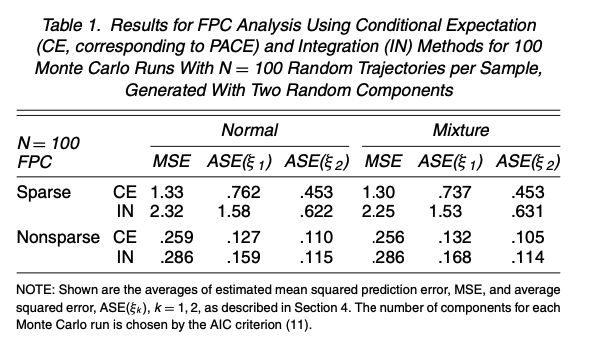
\includegraphics[width=0.48\textwidth]{Figures/Table1.png}
   	\vspace{-0.5 cm}
\end{wrapfigure}

100 iid normal and 100 iid non-normal samples each consisting of $n = 100$ random trajectories were constructed. 
The simulation conditions are: mean function $\mu(t) = t + sin(t)$, and covariance function derived from two eigenfunctions, $\phi_1(t) = -cos(\pi t/10)/\sqrt{5}$ and $\phi_2(t) = -sin(\pi t/10)/\sqrt{5}, 0 \leq t \leq 10$, where $\lambda_1 = 4, \lambda_2 = 1, \lambda_k = 0, k \geq 3$ as eigenvalue and $\sigma^2 = 0.25$ as the variance of measurement errors $\epsilon_{ij}$ (normal with mean 0) in \eqref{eq:eq1}. 
For the smoothing steps, univariate and bivariate Epanechnikov kernel functions were used: $\kappa_1 (x) = 3/4 (1 - x^2) \mathbbm{1}_{[-1, 1]} (x) $ and $\kappa_2 (x, y) = 9/16 (1 - x^2)(1 - y^2) \mathbbm{1}_{[-1, 1]} (x) \mathbbm{1}_{[-1, 1]} (y)$ where $\mathbbm{1}_A (x) = 1$ if $x \in A$ and 0 otherwise.  
For the 100 normal samples, the FPC scores $\xi_{ik}$ were generated from $N(0,\lambda_k)$, whereas the $\xi_{ik}$ the nonnormal samples were generated from a mixture of two normals, $N(\sqrt{\lambda_k/2}, \lambda_k/2) $ and $ N(-\sqrt{\lambda_k/2}, \lambda_k/2)$ with probability $(1/2, 1/2)$.

The performance was evaluated with mean square error (MSE) and average squared error (ASE score). 
$MSE = \sum_{i = 1}^{n} \int_{0}^{10} \left\{X_i(t) - \widehat{X}_i^K(t) \right\}^2 dt/n $; 
$ASE(\xi_k) = \sum_{i = 1}^n (\hat{\xi}_{ik} - \xi_{ik})^2/n$, k = 1, 2. 

\section{APPLICATIONS}

\noindent \textbf{Objectives:} Using PACE, the authors tried to show that they were able 1) to estimate the overall trend over time, 2) to study subject-specific variation patterns, 3) to uncover the dominant modes of variation, and 4) to recover individual trajectories from sparse measurements.

\subsection*{Longitudinal CD4 Counts}
\noindent \underline{Dateset:} A cohort of 283 homosexual men who became HIV-positive between 1984 and 1991 \cite{Kaslow1987}. 
CD4 counts and CD4 percentage, which are markers for the health status of HIV infected individuals, and other clinical tests were recorded.
All individuals were scheduled to have clinical measurements at their semiannual visits. 
However, many individuals missed their visits and the HIV infections occurred at different time points randomly. 
Therefore, the data are sparse and the repeated measurements were irregular. 

\begin{wrapfigure}{r}{0.65\textwidth}
  \vspace{-1 cm}
  \centering
    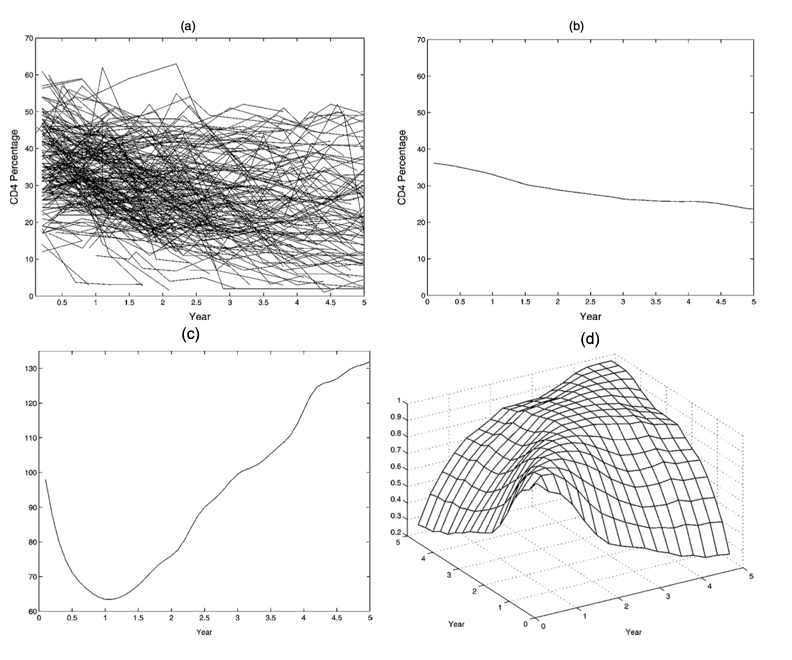
\includegraphics[width=0.64\textwidth]{Figures/Figure1.png}
   	\vspace{-0.7 cm}
   	\caption{(a) Individual trajectories of CD4 percentage in 283 individuals. (b) Smooth estimate of the mean function. (c) Smooth estimate of the variance function for CD4 counts. (d) Smooth estimate of correlation function. }
   	\vspace{-0.3 cm}
	\label{fig:fig1}
\end{wrapfigure}

\noindent \underline{Observations:} 1) The estimate of mean function was able to be build from individual's trajectory. 
From Figure ~\ref{fig:fig1} (b), we can see that the CD4 cell counts are decreasing over a five year course. 

\noindent 2) Variance is non-stationary (decreases at early times and then increase again; see Figure ~\ref{fig:fig1} (c)). 
Correlations between same subjects are strong, but the correlations between early and late CD counts dies off (see Figure ~\ref{fig:fig1} (d)). 

\noindent 3) $K = 3$ was chosen from both one-curve-leave-out cross-validation and AIC, and the resulting three eigenfunctions account for 76.9\%, 12.3\%, and 8.1\% of the total variation. 
Most of the variability is thus in the direction of overall CD4 percentage level.  

\begin{wrapfigure}{l}{0.6\textwidth}
  \centering
    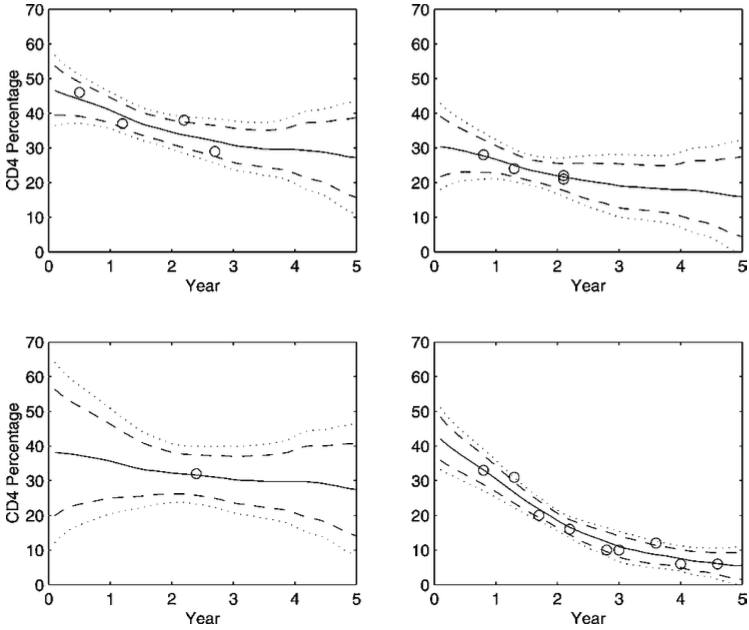
\includegraphics[width=0.59\textwidth]{Figures/Figure5.png}
   	\vspace{-0.5 cm}
   	\caption{Observations (circles), predicted (solid lines) trajectories, and 95\% pointwise (dashed lines) and simultaneous (dotted lines) bands for four randomly chosen individuals, for the CD4 count data.}
	\label{fig:fig5}
	\vspace{-0.7 cm}
\end{wrapfigure}

\noindent 4) The predicted curves and 95\% pointwise and simultaneous confidence bands were shown in Figure ~\ref{fig:fig5}.
It shows that even when the observations per subject is sparse, PACE was still able to effectively recover the trajectories. 
An extreme case was exemplified by the left bottom subfigure, where only one observation was used. 
They showed that they were able to generate reasonably decent trajectory.

\subsection*{Yeast Cell Cycle Gene Expression Profiles}
\noindent \underline{Dateset:} Another dataset the authors used to benchmark their method was the yeast cell cycle data from Spellman et al \cite{Spellman1998}. 
The training set include 6178 genes with each gene expression profile consists of 18 data points, measured every 7 minutes in a span of 0 to 119 minutes. 
The authors artificially induced sparsity to the data by randomly selecting $N_i \; \in (1 - 6)$ with equal probability, and then randomly select from the 18 recorded gene expression measurements (the median of the number of observations per gene expression profile is 3).  %; see Figure ~\ref{fig:fig6}). 

% \begin{wrapfigure}{l}{0.6\textwidth} 
% 	\centering
% 	    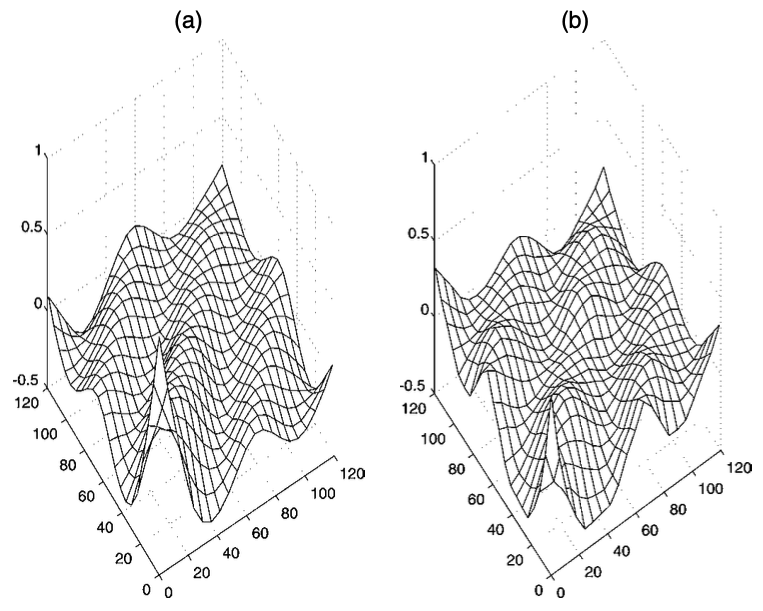
\includegraphics[width=0.59\textwidth]{Figures/Figure7.png}
% 	   	\vspace{-0.5 cm}
% 	   	\caption{Smooth surface estimates $\widehat{G}$ of the covariance functions from the complete data (a) and from the sparsified data (b).}
% 		\label{fig:fig7}
% \end{wrapfigure}

\noindent \underline{Observations:} 1) The mean function estimates for sparse and complete data are close to each other and show periodic features (not shown here).

\noindent 2) The covariance function obtained from complete and ``sparsified'' data set are similar to each other and exhibit periodic features. % (Figure ~\ref{fig:fig7}). 

\noindent 3) The first eigenfunctions were able to approximate the expression profiles (Figure ~\ref{fig:fig8}), which explain approximately 75\% of the total variation.

\noindent 4) 95\% confidence bands were generated using PACE. 
The predictions obtained from the sparse data are similar to those constructed from the complete data (Figure ~\ref{fig:fig8}).

All of these observations demonstrate that the PACE method effectively recover entire individual trajectories from a proportion of the data. 

\begin{wrapfigure}{r}{0.65\textwidth} 
	\centering
		\vspace{-1 cm}
	    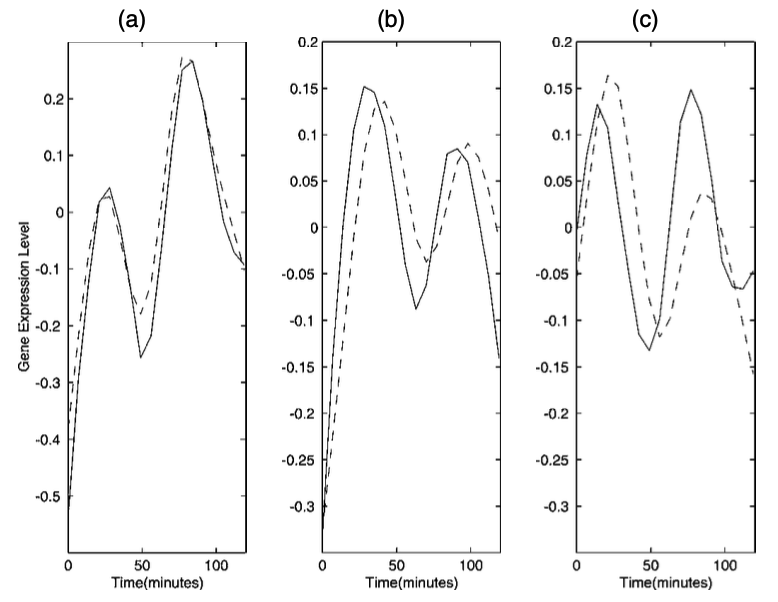
\includegraphics[width=0.64\textwidth]{Figures/Figure8.png}
	   	\vspace{-0.5 cm}
	   	\caption{Smooth estimates of the mean function (a), the first (b) and second (c) eigenfunctions, obtained from sparse (solid lines) and complete (dashed lines) data.}
	   	\vspace{-0.5 cm}
		\label{fig:fig8}
\end{wrapfigure}

\section{CONCLUSIONS}
The authors extended the traditional FPC analysis and developed a method which depends on conditional expectations, which they call ``PACE''.
They showed that PACE was able to handle longitudinal data with irregular measurements and sparse data. 
Using a simulation study and two real-life datasets, they showed that not only PACE effectively recovered the estimation of overall trend of random trajectories, but also allow them to study the subject-specific variation patterns. 
Furthermore, using real datasets, they showed that PACE was able to help impute missing data in longitudinal studies. 
By replacing the integrals by conditional exceptions when estimating FPC scores, PACE improves the traditional FPC analysis under both dense and regular designs. 
This conditional expectation step can be interpreted as shrinkage of the random effects toward 0.  
Overall, PACE shows promise in applications of both longitudinal designs. 


\section{FUTURE RESEARCH}
To make the model more flexible, the authors could investigate extending ``PACE''to additive models. 
The challenge of additive model in functional study could be that the predictor set is not countable and the additive models may require many additive components. 
But because this paper was published a while ago, the authors have done some research on fitting functional additive models \cite{Muller2008}. 
Another area the authors can investigate is how to classify the functional data. 
In practice, it's very often that we need to compare two or more groups of longitudinal data. 
% Another possible research area could be investigating how to estimate the functional gradients of the response with respect to the predictor functions, which would provide quantitative measures of 
% G: $\pmb{z}\sim p_{\pmb{z}} \longmapsto $ Image Space (to generate realistic images)

% \vspace{3mm}
% D: $h\sim p_{data} \longmapsto $ Likelihood (to play an adversarial role)

\newpage
\section*{References}
\printbibliography    



\end{document}
